\documentclass[10pt,twocolumn,letterpaper]{article}

% ကိုယ်ပိုင်အရာများ
\usepackage{booktabs}
% \usepackage{caption}
% \captionsetup[table]{skip=8pt}   % ဇယားများအပေါ်သာ သက်ရောက်သည်
\usepackage{stfloats}  % ဤကို preamble တွင် ထည့်ပါ
\usepackage{float}
\usepackage[T1]{fontenc}

% \usepackage{fontspec}
\usepackage[english]{babel}

% load Lao via babelprovide, turn on "onchar=ids" for automatic shaping
\babelprovide[import,onchar=ids fonts]{burmese}

% main (rm) font for Latin
\babelfont{rm}{Noto Serif}

% Lao text in Noto Serif Lao at 1.2× scale
\babelfont[burmese]{rm}{Padauk}
\babelfont[burmese]{sf}{Padauk}

% alternate (sans-serif) font for Latin
\babelfont{alt}{Lato}

% Lao text in Noto Serif Lao for the alt family too
\babelfont[lao]{alt}{Padauk}

% GPT: LuaTeX doesn’t have built-in Lao line-breaking rules, but babel can assimilate line breaks to hyphenation if you supply some simple “patterns” for common syllable boundaries. Add this to your preamble:
\babelpatterns[burmese]{%
  1က 1ခ 1ဂ 1ဃ 1င 1စ 1ဆ 1ဇ 1ဈ 1ဉ 1ည 1ဋ 1ဌ 1ဍ 1ဎ 1ဏ
  1တ 1ထ 1ဒ 1ဓ 1န 1ပ 1ဖ 1ဗ 1ဘ 1မ 1ယ 1ရ 1လ 1ဝ 1သ 1ဟ
  1ဢ 1ါ 1ာ 1ိ 1ီ 1ု 1ူ 1ေ 1ဲ 1ဲ
  1ျ 1ြ 1ွ 1ှ
  1္ 1့ 1း 1ံ 1်%
}

% \babelpatterns[burmese]{%
%   1က 1ခ 1ဂ 1ဃ 1င 1စ 1ဆ 1ဇ 1ဈ 1ဉ 1ည 1ဋ 1ဌ 1ဍ 1ဎ 1ဏ
%   1တ 1ထ 1ဒ 1ဓ 1န 1ပ 1ဖ 1ဗ 1ဘ 1မ 1ယ 1ရ 1လ 1ဝ 1သ 1ဟ 1ဠ
%   1အ 1ဢ 1ဣ 1ဤ 1ဥ 1ဦ 1ဧ 1ဨ 1ဩ 1ဪ%
% }


\usepackage{cvpr}
\usepackage{times}
\usepackage{epsfig}
\usepackage{graphicx}
\usepackage{amsmath}
\usepackage{amssymb}


\usepackage[breaklinks=true,bookmarks=false]{hyperref}
\cvprfinalcopy % *** ဤလိုင္းကို နောက်ဆုံးတင်သွင်းမှုအတွက် uncomment လုပ်ပါ

\makeatletter
\def\cvprsubsection{\@startsection {subsection}{2}{\z@}
    {8pt plus 2pt minus 2pt}{6pt}{\bfseries\normalsize}}
\makeatother

\def\cvprPaperID{****} % *** ဤနေရာတွင် CVPR စာတမ်း ID ထည့်ပါ
\def\httilde{\mbox{\tt\raisebox{-.5ex}{\symbol{126}}}}

% စာမူတင်သွင်းမှုအဆင့်တွင် စာမျက်နှာအမှတ်ရှိပြီး၊ camera-ready တွင် စာမျက်နှာအမှတ် မရှိပါ
%\ifcvprfinal\pagestyle{empty}\fi
\setcounter{page}{1}
\begin{document}

%%%%%%%%% TITLE
\title{ECDO ဒေတာအခြေခံ ချဉ်းကပ်မှု အပိုင်း ၁/၂: ပင်မအပူထုတ် ကိုယ့်အခန်းခွဲခြားမှု Dzhanibekov လှည့်ချတ်ခြင်း (ECDO) “Earth Flip” သီအိုရီ ၏လက်ရှိနားလည်မှု}

\author{Junho\\
၂ဝ၂၅ ဖေဖော်ဝါရီ တွင် ထုတ်ဝေသည်\\
ဝဘ်ဆိုဒ် (စာတမ်းများ ယူရန်): \href{https://sovrynn.github.io}{sovrynn.github.io}\\
ECDO သုတေသန Git Repo: \href{https://github.com/sovrynn/ecdo}{github.com/sovrynn/ecdo}\\
{\tt\small junhobtc@proton.me}
}

\maketitle
%\thispagestyle{empty}

\begin{abstract}

2024 ခုနှစ် မေလတွင် “The Ethical Skeptic” ဟု အမည်သုံးခဲ့သော အမည်မသိ အွန်လိုင်းစာရေးသူတစ်ဦးက Exothermic Core-Mantle Decoupling Dzhanibekov Oscillation (ECDO) ဟုခေါ်သော အံ့သြဖွယ် သီအိုရီတစ်ခုကို ဝေမျှခဲ့သည် \cite{0,1}။ ဤသီအိုရီအရ ကမ္ဘာမြေသည် ခေတ်သစ်တွင် အကြိမ်ကြိမ် ကြီးမားသော လှည့်ဝင်ဝင်ခြင်းသေတ္တာလှည့်ပြောင်းမှုကြောင့် သမုဒ္ဒရာရေများသည် ကုန်းပြန့်များပေါ်သို့ သိမ်းစီးတက်လှည့်ခြင်းဖြစ်ပွားခဲ့ကြောင်း၊ ထိုအချိန်သည် ကမ္ဘာလှည့်ဝင်ဝကြောင်းတွက်ယူထားသည်။ ထို့အပြင် ဤသီအိုရီတွင် ဂျီဩရေးဗေဒဖြင့် ရှင်းပြချက်တစ်ခုနှင့် ကပ်တိုင်ပြဿနာတစ်ခုနောက်ဘက်ရှိ ဒေတာများပါ တင်ပြသည်။ တကယ်တော့ ဤလို အသျှားသြဇာအလှည့်ပြောင်းမှုများနှင့် ကမ္ဘာအဆုံးသတ် ကြိုတင်ခန့်မှန်းခြင်းများသည် အသစ်မဟုတ်သော်လည်း၊ ECDO သီအိုရီသည် သိပ္ပံဆန်မှု၊ ခေတ်မီမှု၊ အထူးသဖြင့် နည်းကွဲကဏ္ဍစုံနှင့် ဒေတာအခြေခံမှုကြောင့် ထူးခြားစိတ်ဝင်စားဖွယ် ဖြစ်လာသည်။

ဤစာတမ်းသည် ECDO သီအိုရီအပေါ် မျပုံကြီးသုတေသန ခုနှစ်လတာ၏ အနှစ်ချုပ်နှစ်ပိုင်းတွဲထဲမှ ပထမပိုင်းဖြစ်သည် \cite{2,20}။ ထိုသုတေသနမှ အဓိကအချက်သုံးချက်ကို ရှင်းလင်းဖော်ပြထားသည်-

\begin{flushleft}
\begin{enumerate}
    \item ECDO သဘောတူ “ကမ္ဘာလှည့်ပြောင်းမှု” မှသည် လူသားသမိုင်းကြီးအတွင်း ကြိမ်အနည်းငယ်ဖြစ်ပျက်ခဲ့ပြီ ဖြစ်ကြောင်း။ ထို့အထောက်အထားအနေဖြင့် ရေကြီးလေ့လာသုတေသနများနှင့် ကုန်းပြန့်အနှံ့ရေဘေးအောင်မြင်မှု အလံများရှိသည်။
    \item ယခင်က ဖြစ်ခဲ့သော ကမ္ဘာလှည့်ပြောင်းမှု၏ ခန့်မှန်းလားရာနှင့် ပမာဏကို သတ်မှတ်နိုင်သည်။
    \item ကိုယ်တိုင် အနာဂတ်တွင် မကြာခင် “ကမ္ဘာလှည့်ပြောင်းမှု” တစ်ကြိမ် ထပ်မံဖြစ်ပွားနိုင်ကြောင်း၊ ပို၍လည်း မိုးလေဝသလဲလှယ်မှုသည် လူသားများကြောင့်မဟုတ်ဘဲ မြေကြီးအထဲရှိ ပြောင်းလဲမှုမျိုးကြောင့်ဖြစ်နိုင်ကြောင်း၊ ယခင်သုတေသနများအရ အကြောင်းပြချက်များရှိသည်။
\end{enumerate}
\end{flushleft}

ထို့ပြင် ECDO သီအိုရီတွင် အဆိုပြုထားသော “ကမ္ဘာလှည့်ပြောင်းမှု” များနောက်က ရှိသည့် ရှုထောင့်မှုဖိသိပ်မှုဗေဒကိုပါ ပါဝင်ဆွေးနွေး ပြောကြားထားသည်။

ဤစာတမ်းတွင် ငါသည် တရားဝင်ဒေတာများကို အဓိကထားကာ လှုပ်ရှားစိတ်ပျက်စရာအပိုင်းများကို ေရွာင္ရှားလျက် ဤဟာသည် လူသားအနာဂတ်အတွက် ထပ်မံလေ့လာဖို့ အရေးပါတဲ့ အကြောင်းအရာလည်း ဖြစ်ကြောင်း အထူးပြောကြားပါသည်။
\end{abstract}
\section{နိဒါန်း}

မ်ိုးကြီးရေလွမ်းကိစ္စများသည် အသစ်မဟုတ်ပဲ - တကယ်တော့၊ ၎င်းတို့သည် ကမ္ဘာအနှံ့အပြားရှိ ယဉ်ကျေးမှုကြီးတိုင်းတွင်တွေ့ရှိနိုင်ပြီး၊ လူ့ယဉ်ကျေးမှုအစပြုသည့်နေရာတိုင်းတွင် တွေ့နိုင်သည်။ (ပုံ \ref{fig:1}) တွင် ရေလွှမ်းစီးပွားရေးပုံပြင် ၂၆၇ ခုစုစည်းထားသည့်ဒေတာကို ချပြရာတွင် \cite{3} လူနေထိုင်ရာမြေကွက်များအနီးအားလုံးတွင် ရေလွှမ်းပုံပြင်များ တွေ့ရှိနိုင်သည်ကို ဖော်ပြသည်။

\begin{figure}[h]
\begin{center}
% \fbox{\rule{0pt}{2in} \rule{0.9\linewidth}{0pt}}
   \includegraphics[width=1\linewidth]{b.png}
\end{center}
   \caption{ကမ္ဘာအနှံ့ ရေလွှမ်းပုံပြင်များရှိသည့်နေရာများ \cite{3}.}
\label{fig:1}
\label{fig:onecol}
\end{figure}

ဤရေလွှမ်းပုံပြင်များကို နက်နက်မြုပ်မြုပ်ကြည့်လျှင်၊ ၎င်းတို့သည် ပုံမှန်ရေလွှမ်းမှု မဟုတ်ပဲ၊ တကယ်အားဖြင့် တစ်စုတစ်စည်းတည်းတည်းသော ကျောက်တုံးကြီးများနှင့်အတူ အလွန်ဖျက်စီးသော သဘာဝအသီးသီးကြီးမားထိခိုက်မှုအဖြစ် ရေလှိုင်းဖြင့် တစ်ကမ္ဘာလုံးကို သန့်ရှင်းသွားစေသည့်ပြဿနာကြီးများဖြစ်သည်ဟု တွေ့နိုင်သည်။

\subsection{အမေရိကန်ဒေသခံ မုန်တိုင်းပုံပြင်များ}

အမေရိကန်ဒေသခံတို့၏ ပုံပြင်များတွင် ကမ္ဘာ၏ ယောက်ျားကြီးကြီးရေလွှမ်းဒဏ်ကြီးများကို အလွန်တောက်ပြောင်တောက်ပြောင်ရှင်းလင်းစွာဖော်ပြထားသည်။ ဟိုပီ လူမျိုးသည် အနောက်မြောက်အာရီဇိုနာတွင် နေထိုင်သော အမေရိကန် ဒေသခံ လူမျိုးတစ်ခုဖြစ်သည်။ ၎င်းတို့က \textit{"..Sótuknang သည် ကြောင်ရွေပုလင်းတွေကို ရွေးချယ်ထားသော လူတွေကို မြေအောက်မှာ ဝင်ခွင့်ပေးရန် ခေါ်ယူခဲ့သည်။ သူတို့ မြေအောက်မှာ ဘေးကင်းစွာ ရောက်ရှိပြီးနောက်မှာ၊ Sótuknang သည် တောင်ပေါ်၊ မြောက်ခြမ်းနှင့် တောင်ခြမ်း မျက်နှာကျင်းတို့တွင် ကမ္ဘာလည်ပတ်မှုကို ထိန်းသိမ်းရန် တာဝန်ထားခဲ့သော တူညီသောမွေးဖော်စပ်နေသော့များဖြစ်သော Pöqánghoya နှင့် Palöngawhoya တို့ကို ၎င်းတို့၏နေရာများမှ ထွက်ခွာခိုင်းခဲ့သည်။ \textbf{အဆိုပါမွေးဖော်စပ်နေသော့များ မိမိတို့တာဝန်မှထွက်ခွာပါလားလျှင်၊ ထိန်းချုပ်စောင့်ရှောက်သူမရှိသောကမ္ဘာသည် ချောချောမွေ့မွေ့ မတည့်မကျ ဖြစ်လာ၍၊ တစ်ခုတည်းတည်းပဲ လှည့်လည်ပြီး နောက်ဆုံးတွင် နှစ်ကြိမ်လှည့်ကြွေသွားသည်။} တောင်များသည် ပင်လယ်အော်သို့ ကြီးကြီးမားမားကျသွားကြပြီး၊ ပင်လယ်နှင့် ရေကန်တို့သည် မြေပြင်ရှိ ဒေသများသို့ လှိုင်းထူထပ်လာကြသည်။ အဲ့ဒီအချိန်ကမ္ဘာသည် အအေး၊ အသက်မဲ့သော အာကာသတွင် လှည့်လည်သွားရာမှ ရေခဲတုံးကြီးဖြစ်လာသည်"} \cite{4}။
အကြောင်းအရာအမျိုးအစားများမှာ ရေကြီးမှုအဆင့်အတိုင်းအတာကြီးများအား တိတိကျကျဖော်ပြပြီး၊ ပင်လယ်များတက်ကာ တောင်စွန်းအမြင့်ဆုံးများပင် နစ်မြုတ်သွားကြောင်း ဆက်စပ်ဖော်ပြကြသည်။ ဝါရှင်တန်ပြည်နယ်တွင် နေရသော စကိုကိုမစ် လူမ်ိုးများက \textit{"အကြင်နာတော်ကြီးသည် လူနဲ့တိရစ္ဆာန်တို့၏အပြစ်မှုကြောင့် အမျိုးသားတစ်ဦးကောင်း၊ သူ၏မိသားစုနှင့် တိရစ္ဆာန်ကောင်းများကိုသာ ကျန်အောင် ကမ္ဘာ့ပေါ်မှဖယ်ရှားရန် ဆုံးဖြတ်သည်။ အကြင်နာတော်၏ညွှန်ကြားချက်အတိုင်း ထိုသူသည်တစ်လုံးထဲမှမြူလွင်ပြင်တစ်ခုသို့ မြန်မာတစ်လုံးပစ်သည်၊ ထို့နောက် ထိုမြန်မာပေါ်တွင်တစ်လုံးပစ်သည်။ အဲဒီလိုနည်းဖြင့် မိုဃ်းတိမ်မှ မြေထံလာသော မြန်မာကြိုးတစ်စင်းဖန်တီးသည်။ တိရစ္ဆာန်ကောင်းများနှင့် လူကောင်းများသည် စာရင်းတွင်တက်ရန်လုပ်ကြသည်။ တိရစ္ဆာန်ဆိုးများနှင့် မွှေးမြိတ်များသည်လည်း တက်ရန်ကြိုးစားသော်လည်း လူကောင်းသည် မြန်မာကြိုးကို ဖြတ်ပစ်သည်။ \textbf{ထို့နောက်၊ အကြင်နာတော်ကြီးသည် မိုးအများအပြားရွာခိုင်းကာ တာခိုးမာနှင့်တောင်ထိပ်အနီးထိ ရေကြီးစေသည်။} လူဆိုးနှင့် တိရစ္ဆာန်ဆိုးအားလုံး သေဆုံးသွားပြီးနောက်၊ အကြင်နာတော်ကြီးသည် မိုးရွာခြင်းကိုရပ်တန့်စေပြီး၊ ရေများနှေးနှေးကျနင်းလာပြီး၊ လူကောင်းနှင့် တိရစ္ဆာန်ကောင်းများသည် ဆင်းလာကြသည်"} \cite{3} ဟုအကြောင်းပြချက်ပြုကာ ပြောကြသည်။ ဗဟုသုတရရန်၊ တာခိုးမာတောင်သည် ဝါရှင်တန်ပြည်နယ်ရှိ မီးလောင်တက်သောတောင်တစ်လုံးဖြစ်ပြီး ပင်လယ်ရေမျက်နှာပြင်အထက် ၄၃၉၂.၅ မီတာအမြင့်ရှိသည်။

ဝါရှင်တန်ပြည်နယ်ရှိ မကာ လူမျိုးမှ ရေကြီးမှု၏ ဇာတ်လမ်းသည် "အလွန်ပူသော" ရေတွေရေကြီးမှုကြီးမြတ်သော အဆင့်အနည်းငယ်အကြိမ်များလည်း ပါဝင်သည့်အကြောင်းပြုသည်။ ၎င်းသည် ရိုးရှင်းသော ရေကြီးမှုမဟုတ်ကြောင်း ဖော်ပြသည် - \textit{"ပင်လယ်သည် တောင်တန်းဖျားမှဖြတ်တောက်အောင် မြင့်တက်လာသည်။ ထို့နောက် နိမ့်ကျလာ၍ နေရက်ပေါင်းလေးအကြာတွင် နီးယာဘေးသည် အပြည့်အဝခြောက်သွားသည်။ ထို့နောက် ထပ်မံ ပင်လယ်သည်တောင်ထိပါရှိသည့်တောင်ထိပ်မှလွဲ၍ အားလုံးဖုံးလွှမ်းသွားသည်။ \textbf{ထိုတက်လာသည့်ရေများသည် အလွန်ပူသည်။} သင်္ဘောများသယ်ဆောင်ထားသူများသည် သူတို့ပစ္စည်းများနှင့်အတူ အလွန်အနောက်မြောက်သို့ ပို့ဆောင်ခံရကြသည်။ များစွာသောလူများသည် သူတို့သင်္ဘောများ သစ်ပင်တွင်ပိတ်မိသဖြင့် သေဆုံးကြသည်။ နေရက်လေးကြာပြီးနောက် ပင်လယ်သည် နာမည်အတိုင်းပြန်လာကြသည်။ လူများသည် အလွန်အနောက်မြောက်ဒေသတွင် ရောက်ရှိကြသည်။ သူတို့၏မသက်ဆက်များသည် ယနေ့ထိ အနောက်မြောက်တွင် နေထိုင်ကြသည်"} \cite{3}။

\subsection{တရုတ်ပြည်မှ သဘာဝဘေးဇာတ်လမ်းများ}

ပစိဖိတ်မုန်တိုင်းပင်လယ်၏ဖက်တစ်ဖက်ရှိ တရုတ်ယနေ့မြို့ဟောင်းသည် ရေကြီးမှုကြီးတစ်ခုဖြင့် စတင်ခဲ့သည်ဟုဆိုကြသည်။ လကာခေတ်သစ် စတင်ခဲ့သည့်ခန့်မှန်းချက်သည် ခရစ်မေထာပေါ်မတိုင်ခင်နှစ် ၂၀၀၀ ခန့်၊ ယူကြီးကြီးကယ်တင်ရေးကြီးတစ်စုံက မကြာသေးမီကတည်ထောင်ခဲ့သည်။ ယူသည် ကောင်းမြတ္တည်းတို့ အကြီးဆုံးရေကြီးမှုကို ရပ်တန့်စေခဲ့သည်ဟုဆိုသည် \cite{6}။ ၎င်းအချိန်တွင် \textit{"... အံ့သြစရာအဖြစ်အပျက်များဖြစ်ပွားခဲ့သည်။ နေသည်ရက် ၁၀ ခန့်အတွင်း မနေလာတော့ဘဲ၊ တောအုပ်များမီးလောင်သွားခဲ့သည်၊ မမှာမကောင်းတရားရှိသော ပိုးမွှားအမျိုးမျိုးများ ပေါ်လာကြသည်... မျှော်လင့်ရခက်လောက်အောင်ကြီးမားသော ရေလှိုင်းသည် မိုးထပ်ထိမြင်ရလောက်အောင် မြင်ကွင်းကျယ်ပေါ်ပျံကာ တရုတ်ပြည့်သို့ကျရောက်လာသည်။ \textbf{"ရေသည် တောင်မြင့်များထိတက်ရောက်ခဲ့ပြီး၊ တောင်ခြေများသည် အတော်လေး ဖုံးလွှမ်းနေသည်"}... "ရေကြီးမှုအတိုင်းအတာမှာ ဖျက်ဆီးမှုကြီးမားပါတယ်" ဟု မင်းကြီးက ပြောသည်။ "၎င်းတို့သည် တောင်ကူးများ၊ အမြင့်မြတ်သောနေရာများထိကျော်လွှား သို့တိုင်ရောက်ပြီး၊ ရေကြီးမှုကြီးသည် အကောင်းဆုံးတောင်တန်းများထက်တောင် မြင့်တက်သွားသည်။ ထို့ကြောင့် မိမိများသည် တောင်ကြားသို့ ပိတ်ဆို့နေသည့်ရေအတွက်လမ်းထုတ်ရန် ကြိုးစားခိုင်းအပ်ခဲ့သည်။" နှစ်အတော်များများ တစ်နိုင်ငံလုံး လူထုကြီးသည် တောင့်တယ်သောအလုပ်များနဲ့ သယ်ယူဆောင်ရွက်ခဲ့ပြီ။ မြေဆီလွှာများနှင့်ဝန္နယ်များမှ ရေကြီးမှုများ သန့်ရှင်းအောင်ဖယ်ရှားရန် လမ်းချောင်းများတူးရှင်းခြင်းနှင့် လယ်ယာမြေအတွက်ရေကို ဆုတ်ခွာခြင်းစသည့်အရာများ လုပ်ကြသည်။ နှစ်ပေါင်းများစွာ ကြိုးစားမှုအားလုံးအလဟသော်ဖြစ်နေသည်။ ဦးဆောင်သည့် ဝန်ကြီးကွမ်သည် မအောင်မြင်သောကြောင့် သေဒဏ်ချခံရသည်... သူ့သား ယူမှသာ မြေရေကြီးမှုကို ဖယ်ရှားနိုင်ခဲ့သည်။ ဤအောင်မြင်မှုကြောင့် ယူအပေါ် မြန်မာထက်တောင်ချီးမြှင့်သည်။ ထို့နောက် ယူသည် ချွန်မင်းရာထူးရပြီ"} \cite{5}။

တရုတ်ပြည်သည် ရေကြီးမှုကြီးခြင်းသာမက၊ အစွန်းရောက်ဘက်တစ်ခုတွင် ဘေးအန္တရာယ်ကြီးပြီးနောက် ကြယ်တံခွန် နေ့ရက်၊ နေ၊ လ၏လှုပ်ရှားမှုအခြေအနေနှင့် လေးဘက်တည်နေရာများကို ပြန်လည်တိတိကျကျတိုင်းတာရသည်။ ဒါကြောင့် မြေမြန်မြန်လှည့်လှည့်ပြောင်းမှုတစ်ခုဖြစ်ခဲ့နိုင်သည်ဟု ဆိုနိုင်သည် - \textit{\textbf{"ဤမင်းကြီးသည် တရုတ်ပြည်အနှံ့သို့သာမက ဦးမင်းတွင်ပါ မိတ်ဆွေတော်များစွာ ပို့ဆောင်ပြီး၊ နေထွက်နာရီနှင့် နေလင်းနာရီအလိုက် မြောက်၊ အနောက်၊ အရှေ့၊ တောင်တည်နေရာကို ကြည့်ရှုတပ်ဆင်စေလေသည်။} ထို့ကြောင့် မင်းကြီးသည် အချိန်နှစ်ဦးတင်ဖို့ နေရာအချိန်များ စာရင်းပြုစုစေလေသည်... ထို့နောက် ယာူသည် ဟေး၊ ဟိုးတို့အား ဖျော်ဖြေရန်ဘုရင်ကြီး၊ နေ၊ လ၊ ကြယ်တွေ၊ ရာသီလေးခု စသည်ကို မှန်ကန်စွာ စီစဉ်ဖစ်ပေးရန် တာဝန်ထမ်းဆောင်စေလေခဲ့သည်"} \cite{5}။

တရုတ်သမိုင်းမှ သဘာဝဘေးအန္တရာယ်မှတ်တမ်းများသည် လကာမင်းဆက်မစတင်မီ ၃ မင်းနှင့် ၅ မင်းခေတ်တိုင်ကတည်းက ရှိပြီးသားဖြစ်သည် \cite{7}။ နုဝါသည် သုံးမင်းအားလုံးထဲမှ တစ်ဦးဖြစ်ပြီး တရုတ်သမိုင်းတွင် ဖန်တီးမှုအဓိပ္ပါယ်ရှိမှုကြီးတစ်ဦးဖြစ်သည်။ ၎င်းသည် မြေကြီးလှည့်ပြောင်းပြီး သဘာဝဘေးအန္တရာယ်ကြီးဆိုးသောအခါ ရေကြီးမှုတခုကို ရပ်တန့်စေခဲ့သည် - \textit{"အာဏာကြီးသည့် 신အမျိုးအစားနှစ်ဦးအကြား သံသယလုပ်ဖြစ်လို့ တိုက်ပွဲတင်ပြီး ကြီးကြပ်သူရေ신 ဂွုံဂွုံက ရှုံးသည်ကိုမြင်မိလို့ မိုးကွန်တောင်ကို ခေါင်းနဲ့ ထိုးချေလိုက်သည်။ \textbf{တောင်ထောင့်က ဇေယျာထပ်တက်၍ မိုးကောင်းကင်သည် မြောက်အနောက်ဖက်သို့ လှည့်သွားတယ်။ မြေကြီးသည် တောင်အရှေ့ဖက်သို့ ဆက်လှည့်သွားသည်။} ထားရှိ၍ မီးလောင်မှုမဆုံး၊ ရေကြီးမှုကြီးမား၊ လူစားစားစားစားသတ္တိကြီးများပေါ်လာစသည်ဖြစ်သည်။ နုဝါသည် သားအကြီးစားလဲ့တောင်ခြေများဖြတ်ပြီး၊ ပြိုကျသွားသည့်တိုင်ကို အစားထိုးခိုင်းသည်။ နောက်ဆုံးတွင် ကောင်းကင်ကြီးပြတ်သူ အရောင်ဆုံးရောင်မြမ်းများအသုံးပြု၍ ပြန်တွဲသည်။ သို့သော် နုဝါသည် မိုးကောင်းကင်အလှည့်ပြောင်းမှုကို အပြည့်အဝကိုင်တွယ်နိုင်ခြင်း မရှိပါ"} \cite{8}။

\subsection{ဥရောပ၊ မေယန်၊ အလယ်အနောက်၊ အာရှအနောက်တောင်ဘက်မှ သဘာဝဘေးဇာတ်လမ်းများ}

ဤစာတမ်းတွင် ဖော်ပြနိုင်မည့် သဘာဝဘေးဇာတ်လမ်းသည် များစွာရှိသည်။ ထို့ကြောင့် ထင်ရှားထင်မြင်စွာရှိသည့် နိုင်ငံများကို တိုတောင်းစွာသာဖော်ပြပါမည်။ ဂရိစာေပများတွင် ရေကြီးမှုဇာတ်လမ်းသုံးပုဒ် ကြားရမည်ဖြစ်သည်။ ဒေဿူခလီယွန်၊ အော်ဂျစ်၊ ဒားဒါနပ် \cite{9,10}။ ဒေဿူခလီယွန်ဇာတ်လမ်းတွင် \textit{"ရေကြီးမှု ကိုးရက်ကြာပြီးနောက်၊ ကမ္ဘာကြီးဖျက်ဆီးရပ်၍ သင်္ဘောသည် ပါ်နိုက်တောင်၏ထိပ်ပေါ်တွင်ရပ်သည်"}။ ထိုတောင်၏အမြင့်မှာ ၂,၄၅၇ မီတာရှိသည် \cite{11}။ မေယန်စာပေအကောင်းကသုံးသည့် "နေ" များလေးခုတည်ရှိပြီး၊ လက်ရှိ "နေ" မလုပ်မီ စတုတ္ထ "နေ" က ရေကြီးမှုကြီးမှအဆုံးသတ်ခဲ့သည်ဟု ယုံကြည်ချက်ရှိသည်။ ခန့်မှန်းခြေအနေနှင့် ခရစ်မေထာမတိုင်မီ ၃၁၀၀ ဝန်းကျင်တွင် ဖြစ်ပွားခဲ့သည်ဟုဆိုကြသည်။ အလယ်အနောက်တောင်ပိုင်းတွင် ဘာသာရေးသမိုင်းပညာတွင် နုဝမ်၏ ရေကြီးမှုအတေးပြားဇာတ်လမ်းနှင့်၊ ဂီလ္ဂါမက်စ် ဇာတ်လမ်းသည် တူညီသောနည်းအတိုင်း တင်ပြခဲ့သည် \cite{13}။ အာရှအနောက်တောင်ဘက်နိုင်ငံများတွင်လည်း ရေကြီးမှုဇာတ်လမ်းများစွာရှိသည်။ ဥပမာ- အင်ဒိုနီးရှားရှိ အုတ်တန်နှမူ့လူမျိုးတို့သည် \textit{"အကြီးမားဆုံးရေကြီးမှုမှာ လူအများအပြားကို ဒုက္ခပေးခဲ့သည်။ လူအနည်းငယ်သာ ကျန်ရစ်ခဲ့သည်။ သူတို့သည် ရေကြီးမှုမကြီးသော တောင်ထိပ်တစ်လုံးအထိ သင်္ဘောနဲ့အလွတ်တက်နိုင်ခဲ့သည်။ သူတို့သည် ရေလျှောပြတ်သည်အထိ ငါးလလောထိ တောင်ထိပ်တွင် နေထိုင်ခဲ့ကြသည်"} \cite{3}။ ၎င်းတို့နေထိုင်သည့် ဘဝနိုကျွန်း၏ အမြင့်ဆုံးတောင်သည် ၄၀၉၅ မီတာရှိသည်။

\begin{figure*}[b]
\begin{center}
% \fbox{\rule{0pt}{2in} \rule{.9\linewidth}{0pt}}

\includegraphics[width=1\textwidth]{marine.jpg}
\end{center}
   \caption{ကမ္ဘာလုံးဆိုင်ရာ သမုဒ္ဒရာ (သမုဒ္ဒရာ) ဇီဝကျောက်တိုင်များ၊ သနပ်ငန့်ရေ၊ နှင့် ဆားအိမ်/ဆားတူးဖေါက်ရာနေရာများကို ပြသထားသော ပုံပြ မြေပုံ \cite{15,16,86,87}။}
   \label{fig:2}
\end{figure*}

\subsection{အ estadísticas နဲ့ ပျက်စီးမှု ပုံပြင်အနုတ်လက္ခဏာ ချုပ်ဆိုချက်}

ထင်ရှားစွာမြင်ရသည်မှာ၊ ဤပုံပြင်များတွင် မိုးသည်းထန်စွာရွာသောရေကြီးမှုများသည် အခြားသော ဘေးအန္တရာယ်ဆန်သော ဘူမိကမ္ဘာရေးအဖြစ်အပျက်များနှင့်အတူသာလွန်ကျယ်ပြန့်စွာ ဖြစ်ပေါ်နေသည်။ ပျက်စီးမှု ပုံပြင် ၁၁၇ ခု (ဇယား \ref{tab: 1}) ကိုခွဲခြမ်းစိတ်ဖြာသောအခါ မီးတောင်ထွက်မှု၊ မြေမျက်နှာပြင်ပြောင်းလဲမှုများ နှင့် ကမ္ဘာမြေ ခတ်လှည့်မှု ပြောင်းလဲမှုများသည် သံသယတစ်ခုအနေဖြင့် သဲကပ်ရေကြီးမှုကြီးကြပ်မှုနှင့်အတူ ဖြစ်ပေါ်တတ်သည်ဟု မှတ်တမ်းတင်ထားသည် \cite{14}:

\begin{table}[ht]
\begin{center}
\renewcommand{\arraystretch}{1.2}  % Optional, to increase row spacing
\begin{tabular}{|l|c|c|}
\hline
\textbf{ပျက်စီးမှု အမျိုးအစား} & \textbf{အရေအတွက်} & \textbf{ဖြစ်ပွားမှုရာခိုင်နှုန်း} \\
\hline\hline
မိုးသည်းထန်၍ရေကြီးခြင်း/ရေကြီးခြင်း            & ၈၄ & ၇၁.၇၉ \\
မီးလောင်ကျွမ်းမှု/မီးတောင်ထွက်မှု & ၃၉ & ၃၃.၃၃ \\
မြေမျက်နှာပြင် ပြောင်းလဲမှု   & ၂၉ & ၂၄.၇၉ \\
ကြယ်များလှုပ်ရှားမှုအဆင်မပြေမှု           & 15 & 12.82 \\
မိုးကောင်းကင်ပြိုကျခြင်း           & 15 & 12.82 \\
အမှောင်ကြာရှည်စွာတည်ရှိခြင်း      & 14 & 11.97 \\
ပြုတ်မြွေသွားသောမြေဧရိယာများနှင့်တစ်စင်းများ    & 12 & 10.26 \\
လေကျွန်းမုန်တိုင်းများ          & 10 & 8.55  \\
ဝင်ရိုး/လှည့်ပြောင်းမှုများ & 9 & 7.69  \\
ဆူနွေးသောမြစ်များ၊ တစ်စင်းများနှင့်သမုဒ္ဒရာများ & 8 & 6.84 \\
\hline
\end{tabular}
\end{center}
\caption{ပုံပြင်များတွင် ဖြစ်ပေါ်သော ဘေးအန္တရာယ်ကြီးကြပ်မှုများ၏ ဖြစ်ပွားမှုများ}
\label{tab: 1}
\end{table}

ကမ္ဘာတစ်ဝှမ်းရှိ မျိုးစုံသော ယဉ်ကျေးမှုလွတ်လပ်စွာပေါ်ပေါက်လာသော ရေကြီးမှုပုံပြင်များနှင့် အခြား သဘာဝဘေးပြင်းထန်မှုများနှင့်သက်ဆိုင်သော ပုံပြင်များသည်၊ ဤရေကြီးပုံပြင်များမှာ တကယ်တည်ရှိခဲ့သော သဘာဝဘေးအန္တရာယ်များကို တိုက်ရိုက်ဖော်ပြထားခြင်းဖြစ်နိုင်ကြောင်း ပြောသည်။

\section{ပင်လယ်ရေကြီးမှုအတွက် ရုပ်ပိုင်းအထောက်အထား}

ရေကြီးပုံပြင်များနှင့် ကိုက်ညီသော အသီးသီးသော ရုပ်ပိုင်းအထောက်အထားများသည် ကမ္ဘာ့မပါးပြင်ပေါ်တွင် ပင်လယ်ရေကြီးခြင်းများပြားစွာဖြစ်သည့်အထောက်အထားအနေနှင့် တွေ့ရသည်။ အဓိကအထောက်အထားများမှာ ဆား (ငန်ရေ၊ ဆားကန်၊ ဆားမိုင်း) နှင့် ပင်လယ်ရေမွေးဖုန်အရင်းသားများဖြစ်ပြီး ထိုအရာများသည် ကမ္ဘာ့မြေကြီးအတော်လေးရောက်တဲ့ ဧရိယာများကို ဖုံးလွှမ်းထားသည်။ ပုံ \ref{fig:2} တွင် ငန်ရေ (အပြာရောင်)၊ ဆားကန်နှင့်ဆားမိုင်းများ (အညိုရောင်)၊ ပင်လယ်ရေမွေးဖုန်အရင်းသားများ \cite{15,16,86,87} တို့ကို ပြထားပြီး ပင်လယ်ရေကြီးမှု၏ အထောက်အထားများ၏ အကျယ်အဝန်းကို ပြသထားသည်။
Some of the most interesting areas containing saltwater are the Himalayan highlands of Tibet and the Andes mountains of South America, both areas with an average elevation of 4000 meters, the former depicted in Figure \ref{fig:3}. The flood stories of Tibet say that, \textit{"\textbf{တိဘက်ဒေသသည် မတော်တဆ သဘာဝဘေးအန္တရာယ်ကြီးတစ်ခုကြောင့် များပါးစွာရေ မပြည့်လျက်နီးပါးဖြစ်ခဲ့သည်}, ထိုအခါတွင် နတ်ဘုရား Gya သည် အသက်ရှင်ကျန်ရစ်သူများကို ကျေနပ်မူရှိ၍ ရေကို Bengal မှတစ်ဆင့် ဆွဲထုတ်ပေးခဲ့ပြီး လူသားများကို 문명တို့မည့် ဆရာများကိုလည်း ပို့လိုက်သည်၊ ထိုအချိန်ထိ လူသားများသည် ကျားများထက်မကမယ့် တိရစ္ဆာန်တစ်မျိုးသာဖြစ်သည်"} \cite{3}။ ပီရူးဒေသမှ ပုံပြင်များတွင် တောင်တက်လုပ်ငန်းသည် တောင်ထိပ်လှုပ်ရှားမှုအသက်သွင်းမည့် ရေလွင့်မှုကြီးနှင့် တူညီစွာဖြစ်ပျက်သည်ဟု ဆိုသည်- \textit{"သိုးထိူင်းထိမ်းသည်နှင့် သူ့ရဲ႕ ဆဉ်းสาวတိုလေးတို့သည် ရနိုင်သမျှ အစားအစာနှင့် သိုးများကိုစုဆောင်းပြီး အလွန်မြင့်သောအန်ကာစမာကာတောင်ထိပ်ဆီသို့တက်ပို့ခဲ့သည်။ \textbf{ရေလွင့်လာသည့်အခါ တောင်သည်လည်းမြင့်သွားသဖြင့် ထိပ်ရောက်နေဆဲဖြစ်၍ ရေမလွှမ်းသွားခဲ့။ နောက်ကာလတွင်တော့ တောင်သည် ရေနှင့်အတူ အောက်ဆုံးသို့ဆင်းသွားသည်။} ဆဉ်းသားအခြောက်ယောက်သည် ရေလွင့်ပြီးနောက်ပြည်နယ်ကိုပြန်လည်အုပ်စိုးခဲ့သည်"} \cite{3}။

\begin{figure}[t]
\begin{center}
% \fbox{\rule{0pt}{2in} \rule{0.9\linewidth}{0pt}}
   \includegraphics[width=1\linewidth]{tibet.jpg}
\end{center}
   \caption{ဟိမလယအတောင်တန်းမြေပုံတွင် ဆားရေ (အစိမ်းရောင်), ခြောက်သွေ့သည့် ဆားတူးမြေ (အဖြူရောင်) နှင့် ပင်လယ်ရေ ကြည့်ရနည်းတူ ကျောက်မျက်ရတနာ (အနီရောင်)များကို ပြထားသည် \cite{15,16,86,87}။}
\label{fig:3}
\label{fig:onecol}
\end{figure}

While the uniformitarian school of geological thought ascribes anomalies such as salt and marine fossils to drawn-out processes occurring over millions of years, humanity's flood stories should lead us to question that line of thinking. If the ocean really did flood over the continents, then saltwater and marine fossils, easily discovered across vast expanses of high-elevation land, are exactly what we would expect to find.

\begin{figure*}[t]
\begin{center}
\includegraphics[width=0.85\textwidth]{khafre.jpg}
\end{center}
   \caption{တစ်ချိန်ထဲ လူနည်းအတန်ကြာ ပင်လယ်ရေမြင့်တက်မှုကြောင့် ဖြစ်ပေါ်လာသည့် မတူညီသည့် မြေရုပ်ဖွဲ့စည်းမှု နှင့် ပုံသဏ္ဌာန်ရှိသော Karst သဘာဝချွတ်ယက်မှုကို ပြသထားသောဒိုင်ယာဂရမ် \cite{27}။}
\label{fig:4}

\end{figure*}

\subsection{အပိုဆောင်းရုပ်ပိုင်းဆိုင်ရာထူးခြားမှုများ}

အညီသားသဘာဝပညာရှင်များကရှင်းပြလို့မရတဲ့ထူးခြားမှုများအနက် အမျိုးမျိုးရှိပါတယ်။ ထောင်ပေါင်းများစွာနှစ်ကြာပြီးနောက်တောင်အသားစားနိုင်သေးတဲ့အသားနဲ့ညှင်းညပ်ပုံစံခြစ်ထားရင်း၊ ဗြိတိသျှအမဲထီးကြီးတွေကို? \cite{17,18,19} ၊ မြောက်အမေရိကတိုက်မှာ ၂.၄ သန်း စတုရန်းကီလိုမီတာကျယ်ပြန့်စွာတန်းညီညီတန်းတူတည့်တည့်ကျွန်းထည့်ပြီးသဲတန်းတန်းထားတဲ့သည်ကြီးမားသောအလွှာတွေ \cite{21} ၊ မီဂါစီးချောင်းသဲတပ်အကွက်ကြီးတွေနဲ့ \cite{22} ၊ ရာချီကီလိုမီတာအကွာအဝေးကနေလာတဲ့ကျောက်ပြားကြီးတွေတောင်ထိပ်ပေါ်မှာတင်ထားတာတွေ \cite{23,26} တို့က စနစ်တကျသဘာဝပညာရေးဂေါ်လိုဂျီက "ရှည်ရှည်တောင်တောင်ဖြစ်နေတဲ့ဖြစ်စဥ်တွေပဲ" ဆိုတဲ့တခုတည်းသောအကြောင်းပြချက်ကနဲ့ချာချာမြန်မြန်ရှင်းလင်းသွားတဲ့အရာတွေထဲကတစ်ချို့သာဖြစ်ပါတယ်။ ထိုထူးခြားမှုများကို မိုးရွာသဖြင့်ဖြစ်ပွားသောဂြိုဟ်မြေအိမ်သံတို့ဖြစ်တဲ့ဖျက်ဆီးမှုကြီးမားသောဘုံဖိအားများဖြစ်ကြောင်းရှင်းလင်းအကောင်းဆုံးရရှိနိုင်ပြီး၊ ဤစာတမ်း၏ဒုတိယပိုင်းတွင်လည်းဆွေးနွေးထားပါသည်။

ထို့အပြင်၊ သံလိုက်ဧရိယာတောင်ဆစ်ညှိချက်များနှင့်အလှည့်အပြောင်းများသည် ကမ္ဘာမြေအတွက် မကြာခဏထပ်တလဲလဲဖြစ်တတ်သည်ဟု ပဲလီယိုသံလိုက်ဒေတာအပေါ် မှီငြမ်း၍ ကျယ်ပြန့်စွာလက်ခံလျက်ရှိကြသည် \cite{35,40,41} ။ သို့သော်၊ ခေတ်သစ်သိပ္ပံသည် ထိုအလှည့်အပြောင်းများ မည်သို့၊ မည်သည့်အကြောင်းကြောင့် ဖြစ်ပွားသည်ကို မရှင်းပြနိုင်ပေ။

\section{ECDO နှင့် Giza ၏ပီရမစ်များ}

Giza ၏ Khafre နှင့် Khufu ပီရမစ်များသည် Ethical Skeptic ၏ ECDO သီအိုရီအတွင်း အဓိကအချက်အချာအနေဖြင့်ပါဝင်သည် \cite{27} ။ အဆိုပါပီရမစ်များသည် တာကျပ်သည့်ယာယီသမုဒ္ဒရာရေလှုပ်ရှားမှုပြဿနာများကိုသက်သေပြနေသလို၊ ကမ္ဘာမြေအပေါ် ECDO ပြောင်းလဲမှုများ၏အရိပ်အမြွက်ကိုလည်းညွှန်ပြသလိုမြင်ရသည်၊ ဒါ့အပြင် ကျွန်ုပ်တို့၏ဘိုးဘွားများသည် ကမ္ဘာမြေအပျက်အမြှောက်များကိုတိုင်းတာနိုင်ပြီး ထိုသတင်းအချက်အလက်ကို ကြီးမားစွာဖြစ်վող ကျောက်တုံးအဆောက်အဦးများအတွင်း ထည့်သွင်းရိုက်နှိပ်နိင်ခဲ့ကြသည်ဟုလည်းဆိုနိုင်သည်။ ဤပီရမစ်နှစ်ဆူသည် ခန့်မှန်းခြေ ခန့်သတ်ရင် ခုနစ်တစ်ထောင် B.C.E အနီးမှာ Khufu နှင့် Khafre ဘုရင်များအတွက်သေရေအိမ်အဖြစ်တည်ဆောက်ခဲ့သည်ဟု ယုံကြည်ကြသည်။ ထိုအဆောက်အဦးများသည် မြောက်အီဂျစ်၏ (၃၀ မြောက်လတ္တီတွဒ်၊ ၃၁ အရှေ့လောင်ဂျီတွဒ်)ခန့်တွင် တည်ရှိပြီး၊ အုတ်တိုင်းရင်ပေါ်အရ တစ်ခုလျှင် ၂၀၀ မီတာကျော်ရှိသည်၊ အမြင့်မှာလည်း ၁၄၀ မီတာခန့်ရှိသည်။ Khufu ပီရမစ်ကို ဝကျောက်အုပ်ကာလประมาณ ၂.၃ သန်းခန့်အသုံးပြုခဲ့ပြီး၊ တစ်ခုချင်းစီသည်ပျမ်းမျှနှစ်တန်ကျော်လောက်ရှိသည် \cite{24, 25}။

ဤပီရမစ်များ၏ မူလအစအနောက်တွင် အတည်မပြုနိုင်သည့်တိကျချက်ကြီးမားစွာရှိနေသည်ကို Ethical Skeptic ၏စာတမ်းတွင် လောင်လောင်ထိုးထိုးဖော်ပြထားသည်။ ယင်းသည် ပီရမစ်များနှင့်ပတ်သက်သည့်ပုံမှန်အဓိပ္ဘာယ်တွင် ညီညွတ်မှုမရှိမှုများအဖြစ် များစွာထုတ်ဖော်ပြသထားပြီး၊ မနည်းလူသိရှားကြားသောသက္ကရာဇ်နှင့်သမိုင်းကြောင်းအပေါ် တွေ့ကြုံနေရသည်ဟု၎င်းပြောသည် -

\begin{flushleft}
\begin{itemize}
    \item အနီးအနားရှိစုစစ်ဟောင်းမွေးစားထားသည့်အင်္ကျီသစ်များနှင့်လုယက်သူလုပ်ငန်းသုံးကိရိယာများကို ကားဘွန်ရက်တည်ဖြင့်စမ်းသပ်သည့်အခါ ပီရမစ်တွေကို ယနေ့လူသိအတိုင်းထက်ပိုပြီးရှေးကတည်ဆောက်ခဲ့ကြောင်း ပြသသည်။
    \item Khufu ပီရမစ်အတွင်းရှိဆိုကြသည့်မုန့်သုတ်ဖြစ်သော တူးယူကန့်သတ်ထားသည့် အမှတ်အသားများတွင်၊ ၎င်းတို့ထားရှိမှုနေရာ၊ အသုံးပြုသောပစ္စည်း၊ ထိန်းသိမ်းမှုအခြေအနေ၊ အီဂျစ်အက္ခရာအသုံးပြုမှု၊ ရှာဖွေတွေ့ရှိချိန်နှင့်လက္ခဏာများသည် သံသယဖြစ်စရာများစွာရှိပြီး၊ ၎င်းတို့သည် ဖြောင့်မြည်သည့်လုအိတ်ဖြစ်နိုင်ကြောင်းပြသသည်။ ထိုသိမ်းထားသည့်အမှတ်အသားများသည် ပီရမစ်၏ တစ်နေရာတွင်တွေ့ရှိသော အစစ်အမှန်သက်သေအနက်နဲ့ သဘာဝရာသီလက္ခဏာဟောင်းတွေကွဲပြားသည်။
    \item နီးစပ်သော Sphinx ပေါ်ရှိ ထူးခြားစွာ ကာစ်တူးယစ်ပျောက်ရန်မော်တော် အွမ်းမှုသည် ပုံမှန်အကျင့်နှင့် မကိုက်ညီပါ။
\end{itemize}

\end{flushleft}

\begin{figure*}[b]
\begin{center}
\includegraphics[width=0.85\textwidth]{shafts.jpg}
\end{center}
   \caption{Khufu ပီရမစ်၏ အတွင်းပိုင်း လှေခါးများနှင့် အခန်းများကို ပြသထားသည်။ Ethical Skeptic မှ ရည်ညွှန်းသည်မှာ ဒါဖြစ်ကောင်းပါက ၎င်းသည် ECDO ဖြစ်ရပ်များအတွက် အပိုင်းသုံးပိုင်း ပါဝင်သော ဒေသဆိုင်ရာ ဘူမိကြောင့် ဖြစ်ပေါ်သော ရေကြောင်း အနီတိရှိသော စောင့်ကြည့်သည့် နည်းပညာရုံတစ်ခုဖြစ်သည်ဟုဆိုသည် \cite{28}။}
\label{fig:5}
\end{figure*}

Ethical Skeptic ၏ သုတေသနအချက်လက်အနက်တစ်ခုမှာ ပုံ \ref{fig:4} တွင် ပြထားသည့် Khafre ပီရမစ်၏ ပြင်ပ မညီညာသော စနစ်တကျ ရေချိုးဖျက်မှု ဖြစ်ပါသည်။ ပီရမစ်တောင်ထိပ်တွင် မူလ Tura အလွန်ပျော့သော မာကျောက်ဂွမ်းအပြင်အပေါ်တပ်ဆင်ထားသော အလွှာကို ထိန်းသိမ်းထားပါသည်၊ ၎င်းသည် ပီရမစ်တစ်လုံးလုံးကို မတခင်အထိဖုံးလွှမ်းထားသည်။ ဤ မာကျောက် ဂွမ်းအလွှာ ထိပ်သည် နူးညံ့စွာ ရာသီဉတုသက်တမ်းရေစားတက်သော်လည်း မိမိအောက်တွင် တင်းမာတည့်ငြိ MoHS 7 Mokkatam မာကျောက်ဖြင့် ပြုလုပ်သည့် ပီရမစ်အတွင်းဖွဲ့စည်းပုဒ်များရှိသည့် အလွန်ကြိမ်ခန့်ကပ်စိမ့်ကျတဲ့ ချွေးခြောက်သော အလွှာတစ်ခုမှ တိုက်ရိုက်ရှိပါသည်။ ၎င်းအောက်တွင်တော့ ပီရမစ်ကိုယ်တိုင်မှာ အလွန် ချွေးခြောက်သည့် MoHS 4 Tura မာကျောက်အလွှာဖြင့် ရှိသည်။ ဤနေရာတွင် အဓိကအချက်မှာ ပီရမစ်၏ ပြင်ပအလွှာအဖြစ် သုံးခဲ့သော ပျော့သော Tura မာကျောက်သည် CaCO$_3$ ဖြစ်ပြီး မှန်ကန်သောအခြေအနေထဲ၌ရေဖြင့် လွယ်ကူစွာပျော်သည်။ Ethical Skeptic သည် ချွေးခြောက်ခြင်းအလွန်ပြင်းထန်သည့် အလွှာသည် တင်းမာသော Mokkatam မာကျောက်တွင် ရပ်တံ့မှု၊ ထိပ်ထောင့်များတွင် လှိုင်းပုံစံ ရေချိုးဖျက်မှု၊ ထောင်ခြင်းမှနားထောင်သည့် ထိပ်၏ နူးညံ့သက်တမ်းရေစားခြင်းနှင့် ပီရမစ်အောက်ပိုင်း၏ ပြင်းထန်သော ချွေးခြောက်ခြင်းအကြား ကွာခြားချက်တို့ကို မြင့်တက်လာပြီး ချက်ချင်းပြန်လျှော့သွားသော သမိုင်းကာလတလျောက် ပင်လယ်ရေမိုက် တက်လာမှုကို သက်သေပြသော အထောက်အထားရှင်းရှင်းလင်းလင်းအဖြစ် ညွှန်ပြထားသည် \cite{27}။

\begin{figure*}[b]
\begin{center}
% \fbox{\rule{0pt}{2in} \rule{.9\linewidth}{0pt}}
\includegraphics[width=1\textwidth]{drawing.jpg}
\end{center}
   \caption{31$^\circ$ အရှေ့ လောင်တီကျုတော်တော်လှန်လျှောက်တစ်လျှောက် 104 ဒီဂရီ မြောက်ဖက်သို့ လှည့်ခွင့်ရသော ECDO လှည့်ပတ်မှု ကို ပုံဖော်ပြသထားသည်။ ချက်များသည် အရှေ့နှင့် အနောက် လှည့်ဝိုင်းတိုင်များကို ပြပြီး အနီရောင်အမှတ်သည် Khufu ပီရမစ်ကို သရုပ်ပြသည်။}
\label{fig:6}
\end{figure*}
Ethical Skeptic အနေနဲ့ Khufu ပီရမစ်အတွင်းပိုင်း ဒီဇိုင်းနဲ့ အခြေအနေနှင့် ပိုမိုဆက်စပ်ပြီး သူ့ရဲ့ စုံစမ်းစစ်ဆေးမှု (ပုံ \ref{fig:5}) မှာ အလေးထားလေ့လာထားပါတယ် \cite{28}။ Khufu ပီရမစ်ထဲမှာ အခန်းတချို့ (မင်းသားကြီး၊ မင်းသမီးကြီးနဲ့ မြေအောက်အခန်းတွေ)၊ လမ်းကားတွေနဲ့ မြောင်းလမ်းတွေအပြင်၊ "လေထွက်ပေါက်" လို့ခေါ်တဲ့ မောင်းစုံ နှစ်စုံလည်းပါဝင်ပါတယ်။ တစ်စုံဟာ မင်းသားကြီးအခန်း၊ တစ်စုံက မင်းသမီးကြီးအခန်း‌မှ များထွက်နေပါတယ် \cite{29,30}။ ဒီစာတမ်းမှာတော့ Ethical Skeptic ရဲ့ စုံစမ်းမှုထဲမှာ အရေးကြီးဆုံးအပိုင်း — "လေထွက်ပေါက်" နှစ်စုံရဲ့ တည်နေရာနဲ့ ဒီဇိုင်းကိုသာ တစ်ခုထဲဖော်ပြပါမယ်၊ မPorque Earth ရဲ့ ECDO ပြောင်းလဲမှုအကြောင်းအရာ အရေးပါသော ಮಾಹಿತಿများ စာတန်းထဲမှာ တင်ထားလို့ပါ။

ဤနေရာမှာသော့ချက်မှာ လေထွက်ပေါက်များသည် တိကျသော ဦးတည်မှုတစ်ခု ချထားခဲ့ကြောင်းကို နားလည်ရမှာဖြစ်ပါတယ်။ ပထမတစ်ခုကတော့ လေထွက်ပေါက် နှစ်စုံလုံးဟာ ယခုအချိန်မှာ အရှေ့မြောက်နှင့် တောင်ဘက်ကို တိုက်ရိုက် ဦးတည်နေပါတယ်။ ထို့အပြင် တစ်စုံခြင်းစီမှာ ၁၀၄ ဒီဂရီ ထောင့်ဖြင့် တည်ဆောက်ထားပါတယ်။

အရေးကြီးဆုံး သက်သေကတော့ မင်းသမီးကြီးအခန်းထဲက လေထွက်ပေါက်တစ်ခု၏ အတွင်းမှာ ရိုက်ထုထားသော အလံကြယ်မြေပုံတစ်ခုပါ။ ဒီအလံကြယ်မြေပုံက ပြိြိုင်သာဘက်စွဲ့အလယ်ဗဟိုနဲ့ (ယခင်လကာလအနီး ၉၆၀၀ မှ ၉၂၀၀ BCE) ပတ်သက်နေပါသည်။ ဒီအရာက လေထွက်ပေါက်မှ တည်နေရာထားမှု သေချာစွာ ချထားခဲ့ကြောင်းနဲ့ တည်ဆောက်ချိန်မှာ မင်းသားကြီးနဲ့ မင်းသမီးကြီး အခန်းထဲက လေထွက်ပေါက်နှစ်ခုက ပြိြိုင်သာဘက်စွဲ့ကို ဦးတည်ထုတ်ထားကြောင်းဆောင်ကြဉ်းပေးပါတယ်။ ဒါဖြင့် မျှော်လင့်ချက်တစ်ခုဖြစ်လာပါတယ်။ — လေထွက်ပေါက်တစ်ဖက်စီက ဘာကို ဦးတည်နေသလဲနှင့် ဘာကြောင့် ၁၀၄ ဒီဂရီထောင့်နဲ့ တည်ဆောက်ကြတာလဲ။ Ethical Skeptic က ဒီများကို ၁၀၄ ဒီဂရီ ECDO ပြောင်းလဲမှုနောက်ကြယ်မြေပုံအတိုင်း ပြိြိုင်သာဘက်စွဲ့ကို ဦးတည်စေဖို့ တည်ဆောက်ခဲ့ကြောင်း ခန့်မှန်းပါတယ်။

\section{၃၁ ဒီဂရီ မြားလိုင်းတလျှောက် ၁၀၄-ဒီဂရီလှည့်ခြင်းအတွက် သက်သေများ}

Ethical Skeptic ကတော့ မြေမြတ်သည် ၃၁‌ ဒီဂရီမြားလိုင်းအတလျှောက် တစ်ခါခြင်းတစ်ခါ ၁၀၄ ဒီဂရီ လှည့်မှုများရှိကြောင်း၊ အဲဒီလိုင်းပေါ်မှာဘဲ Khufu ပီရမစ်နဲ့ ခုနှစ်နှစ်ချင်းလေထွက်ပေါက်တွေတည်ရှိကြောင်းအဆိုပြုသည်။ ပုံ \ref{fig:6} မှာ ခန့်မှန်းထားသည့် လှည့်မှု၊ အရှေ့ဘက် (အင်ဒိုနီးရှား ၁၂၁ ဒီဂရီအရှေ့လှည့်) နှင့် အနောက်ဘက် (တောင်အမေရိက ၅၉ ဒီဂရီအနောက်လှည့်) "ထောက်ကန့်", အဲဒီ ၂ နေရာကတော့ ၃၁ဒီဂရီမြားလိုင်းအတလွှောက် လှည့်သွားတာနောက်မှာ တည်နေရာမပြောင်းဘူး။ မြေမြတ်က ဒီအခြေအနေသစ်ကိုရောက်နောက်မှာတော့ (တစ်ဆယ်စုနှစ်တစ်ချိန်မှ စတုတျမာန်တိုင်အောင်) အနည်းငယ်ပြန်ကြာသေးမယ်ဆိုသည် \cite{150}။

အလွန်တည့်သောဘေးအန္တရာယ်ဇာတ်လမ်းတစ်ပုဒ်က ယဉ်ကျေးမှုအဖြစ် အထင်ကရဆုံး ဂရိမှ သမိုင်းရေးရာအတော်ဆုံးဖြစ်သည့် Herodotus မှ ပြောပြထားသောခေတ်သမိုင်းတှေ့ ဖြစ်သည်၊ သူသည် မေရိစ်ခေတ်ငယ် ၅ ရာစု မှာနေထိုင်သူဖြစ်သည် \cite{31}။ သူ့ရဲ့ "An Account of Egypt" ဆိုတဲ့စာအုပ်ထဲမှာ Herodotus က ဗြိတိသျှက သူ့ကိုပြောပြခဲ့သည့်အတိုင်း \textit{"...ပထမ မင်းစတင်ပြီး ဒီ Hephaistos ဘုရား၏ ကျောင်းသားမင်းနောက်ဆုံးစိုးစော်ခဲ့ချိန်အထိ လူသားမျိုးဆက် ၃၄၁ ဆက်ရှိခဲ့ကြောင်း... သို့သော် လူမျိုးဆက် ၃၀၀ ဆိုတာ ၁၀,၀၀၀ နှစ်တန့်၊ အကြောင်းမှာ လူမျိုး ၃ ဆက်ဆိုရင် နှစ် ၁၀၀ ဖြစ်တယ်... ထို့နောက် ၁၁,၃၄၀ နှစ်ကာလအတွင်း ဘုရားတစ်ပါးမှလည်းလူ့ပုံစံနဲ့လာခြင်းမရှိပါ၊ ထို့အပြင် ဗြိတိသျှတွေထဲမှာတောင် မင်းများထဲကမည်သို့မျှ မဖြစ်ပြသန်ပါဘူး။ \textbf{ဒီ ခုနှစ်တွေမှာ နေရောင်က သူ့ရဲ့ မီအာဝင်ထုံးစံနေရာကနေ လေးကြိမ် ပြောင်းပေးခဲ့ရတာ၊ ယခုနေရောင်ကြယ်တောင်ဘက်ကနေ နှစ်ကြိမ် ထောင်နေရုံ၊ အရှေ့ဘက်ကနေ နှစ်ကြိမ်ဆင်းနေရုံ ဖြစ်သည်;} တစ်ချိန်ထဲမှာတော့ ဧဂျစ္ပ့်မှာ ဘာမှ၊ မြေနဲ့ပတ်သက်သည်တစ်ခုတည်းပဲ၊ မြစ်ရေ၊ ကူးလာတဲ့ရောဂါ၊ သေခြင်းတို့ ဘာမှ မပြောင်းလဲပေ"} \cite{32}။ Hephaistos ဘုရားကျောင်းသားမင်းကတော့ မြောက်အာရှစည်သူ Sennacherib နဲ့ တစ်ဦးတည်း ခေတ်သူဖြစ်တာကို Herodotus မိမိကတင်ပြထားသလို (ရွေးချယ်ချက်တို့မှာ) ခုနစ်ခုနှစ်၈ရာစုအစောပိုင်းတွင် ရှေးခေတ်စားနိုင်ပါတယ် \cite{32,33,34}။

ဒီဇာတ်လမ်းက အရေးကြီးချက်ကတော့ နှစ်ထပ်တိတိနေရောင်ကြယ်က ဧဂျစ်မှာ လောင်နေတဲ့နေရာနဲ့ ဆင်းနေတဲ့နေရာ ပြောင်းလဲခဲ့ကြောင်းကို ပြောပြတာပါ။ ဒါက ဧဂျစ်က ၁၈၀ ဒီဂရီ ပြောင်းသွား၊ latitude မှာတော့လည်း မပြောင်းဘူးဆိုမှသာ ဖြစ်နိုင်ပါတယ်။ ပီရမစ် ဒီဇိုင်းနဲ့ နောက်တစ်ပိုင်းမှာ ပြောမယ့်ဒေတာတွေကို တွဲတွေးကြည့်ရင် ဧဂျစ်ဟာ မြေမြတ်သစ်လိုက်တဲ့ မြားလိုင်းပေါ်မှာ တည်ရှိနေနို်င်တယ် (၃၁ ဒီဂရီအရှေ့မြားလိုင်း) ဖြစ်တယ်ဆိုတာ သေချာပါတယ်။

ဧဂျစ်ကတစ်ဦးတည်းသော နေရောင် ရှုထောင့်ပေါ်မှ ထူးခြားသည့် ပြောင်းလဲမှုကြောင့် ဇာတ်လမ်းတစ်ပုဒ်ရှိတဲ့နေရာပဲ။ မျှတစွာမြေပြားလှည့်မှု ဦးတည်ရာအရင်းအမြစ်ပြောထားတဲ့ တခြားတစ်ခုက တရုတ်မင်းမကြီး Nüwa ဇာတ်လမ်းဖြစ်ပြီး၊ \textit{"မင်းတိုင်က ပြိုကျသွားပြီး မိုးက နောက်ကွယ်နောက်အောက်ဘက်ကို နိမ့်ချပြီး မြေဆောင့်က တောင်အရှေ့ဘက်ကို "ချိုး" ဆုတ်လှည့်သွားသည်"} \cite{8} ဟုရေးထားသည်။ ဒီလှည့်မှုဦးတည်ရာကလည်း ဤစာတမ်းအဖြစ်အပျက်နဲ့ ကိုက်တွယ်ပါတယ်။

\subsection{၃၁ ဒီဂရီ မြားလိုင်းတလျှောက် ၁၀၄-ဒီဂရီ လှည့်မှုအတွက် ရုပ်ပိုင်းဆိုင်ရာ သက်သေများ}

ဒီလှည့်မှု ဦးတည်ရာကိုထောက်ပြနိုင်တဲ့ ရုပ်ပိုင်းဆိုင်ရာ သက်သေအထောက်အထားတွေထဲမှာ သံလိုက်အဟုန်၊ တစ်တိုနစ်၊ သဲကန္တာရ၊ တောတိရစ္ဆာန်မျိုးစုံအာ့တေ့၊ မြစ်ရေစီးအနံ့၊ နှင်းတောင်တက်ခဲလှေသည်များ ပါဝင်သည်။
A study of paleomagnetic data preserving the geomagnetic pole paths of the Iceland Basin and Laschamp excursions \cite{35}, depicted in Figure \ref{fig:7}, shows the poles rotating approximately around the eastern ECDO pivot of (0 N, 121 E). This data is recorded in certain kinds of magnetic minerals in rocks that formed during the pole excursions, preserving information about the direction and intensity of the Earth's magnetic field at that time.

\begin{figure}[t]
\begin{center}
% \fbox{\rule{0pt}{2in} \rule{0.9\linewidth}{0pt}}
   \includegraphics[width=0.95\linewidth]{laj.jpg}
\end{center}
   \caption{အိုက်စ်လန်ဘေစင် လှည့်လည်သွားသည့် ဂျီယိုမဂ္နီတစ်ဘောလုံးစက်ဝိုင်းလမ်းကြောင်း (a) နှင့် Laschamp လှည့်လည်မှု (b) အတွက် မျိုးမတူ ဂျီယိုမဂ္နီတစ်ဘောလုံးစက်ဝိုင်းလမ်းကြောင်းများ \cite{35}။}
\label{fig:7}
\label{fig:onecol}
\end{figure}

\begin{figure}[t]
\begin{center}
% \fbox{\rule{0pt}{2in} \rule{0.9\linewidth}{0pt}}
   \includegraphics[width=1\linewidth]{meinesz3.jpg}
\end{center}
   \caption{ကမ္ဘာမြေမူဘောင်အတွင်း ရွှေ့ပြောင်းထူထောင်မှု ပုံစံများကို ဖော်ပြထားခြင်း \cite{36}။}
\label{fig:8}
\label{fig:onecol}
\end{figure}

\begin{figure*}[t]
\begin{center}
% \fbox{\rule{0pt}{2in} \rule{.9\linewidth}{0pt}}
\includegraphics[width=0.95\textwidth]{biodiversity.jpg}
\end{center}
   \caption{ကမ္ဘာ့အကြီးဆုံး သဲမြေများနှင့် အလှပဆုံး သဘာဝဇီဝပေါင်းစုံ ရှိရာဒေသများကို ဖော်ပြထားသည် \cite{28}။}
\label{fig:9}
\end{figure*}

ကမ္ဘာမြေထဲရှိ ချိုင့် (မူကြမ်း) များကို လေ့လာခြင်း (ပုံ \ref{fig:8}) တွင်၊ ကမ္ဘာ့မြေခွဲများ ပျက်စီးမှု သို့မဟုတ် အနာကြီးခြင်းဖြစ်သည့်နေရာများတွင်လည်း အတူတူပုံစံကို တွေ့နိုင်သည်။ ဒတ္ချ် လေ့လာပညာရှင် Felix Meinesz သည် သူ့စာတမ်း \cite{36} တွင် ဤပုံစံ ဖြစ်ပေါ်သည့် အဓိကအကြောင်းရင်းမှာ ကမ္ဘာ့လည်ပတ်မှတ်ဉီးတည်ချက်ပြောင်းလဲမှု ဖြစ်နိုင်ကြောင်း ရှင်းပြထားသည်။

ကမ္ဘာ့အကြီးဆုံး သဲမြေများနှင့် သဘာဝဇီဝပေါင်းစုံ သိပ်သည်းသော ဒေသများလည်း ဤပုံစံနှင့် ကိုက်ညီမှုရှိသည်။ သဲမြေများသည် အမဲလွှမ်းမိုးမှုကြီးမားစွာ ခန့်မှန်းခံရသောနေရာများတွင် ရှိနေပြီး၊ သဘာဝဇီဝပေါင်းစုံ သိပ်သည်းသောဒေသများသည် ပင်လယ်ရေရွှံ့ပြောင်းမှုမှ မပြင်းထန်စွာ ထိခိုက်ခြင်း မရှိသောနေရာများတွင် ရှိနေသည် \cite{28}။ ဤကိုက်ညီမှုအား ပုံ \ref{fig:9} တွင် ဖော်ပြထားသည်။

ခန့်မှန်းထားသော ECDO လည်ပတ်ခြင်းလမ်းကြောင်းနှင့် ကိုက်ညီနေသည့်စဥ်းမျဉ်းများသည် အမေရိကန်အနောက်ပိုင်းရှိ သဲတောတန်းအလွှာများတွင်သိမ်းဆည်းထားသော ငါးသလောက်နဲ့သဲသဲသားရေလှိုင်းများ (paleocurrents) နှင့်သက်ဆိုင်သည် \cite{21}။ ထို့အပြင်၊ ရေခဲတောင်ကြီးများက ယူဆရသည့် စွန့်ပစ်ကျောက်တုံးများဖြစ်သည့် glacial erratics များသည် မူရင်းကျောက်မျက်ရဲ့မတူကွဲပြားသော မူခိုးစက်နှင့်အတူတစ်ခြားကျောက်မျက်ပေါ်တွင် စွန့်ပစ်ထားရသော ထင်ဟပ်ကျောက်များဖြစ်သည်။ ဗြိတိန်နိုင်ငံတွင် ဤက်တောက်ကျောက်များသည် ECDO လည်ပတ်ခြင်းနှင့်ကိုက်ညီသော စီးဆင်းမှုလမ်းကြောင်းနှင့် ကိုက်ညီသည် \cite{67,68}။

\section{ECDO ပြောင်းလဲမှု၏ ဖြစ်ပေါ်စေသည့် ရူပဗေဒပညာ}
\begin{figure*}
\begin{center}
% \fbox{\rule{0pt}{2in} \rule{1\linewidth}{0pt}}
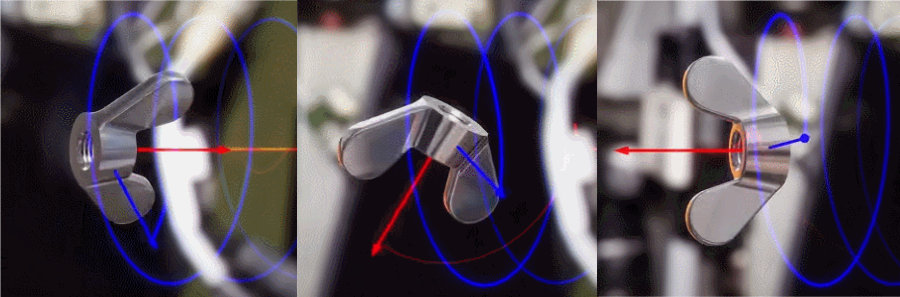
\includegraphics[width=0.9\textwidth]{dzhani.jpg}
\end{center}
   \caption{Dzhanibekov အကျိုးသက်ရောက်မှုကို ဖော်ပြချက် \cite{28}။}
\label{fig:10}
\end{figure*}

မြေပြင်လှည့်လည်မှု ဝင်ရိုးတစ်ခု အလွန်မြန်မြန် ပြောင်းလဲခြင်း၏ အခြေခံအစွမ်းသတ္တိသည် လှည့်လည်နေသော ခုန်ပစ္စည်းများ၏ ရူပဗေဒအပေါ်မှာ မူတည်သည်။ ၎င်း၏ ရိုးရာ ဥပမာမှာ Dzhanibekov အကျိုးသက်ရောက်မှု ဖြစ်ပြီး ရုရှား အာကာသယာဉ်မှူး Vladimir Dzhanibekov မှ ရှာဖွေတွေ့ရှိခဲ့သည် \cite{37}၊၊ နောက်ဆုံးတွင် ဓာတ်ပုံ \ref{fig:10} တွင် ဖော်ပြထားသည်။ ခုန်ပစ္စည်းတစ်ခုသည် ၎င်း၏ အင္အားလျှပ်စစ်သွား ဝင်ရိုးသုံးခုထဲမှ တစ်ခုမှာ စုံသည့် လှည့်လည်မှု မရှိပါက ဝင်ရိုးတစ်ခုကို တည်တစ်ရာ မပြုနိုင်ပါ။ ၎င်း၏ ဒုတိယ ဝင်ရိုးအနီးတွင် လှည့်လည်နေပါက သတိပြုမိနိုင်သည့် ထောင့်အရပ် လှည့်ပြောင်းမှုမြန်မြန် ဖြစ်ပေါ်လာနိုင်သည်။ ဒါပေမယ့် ယင်းသည် မြေကမ္ဘာ၏ လှည့်လည်မှု မြန်မြန်ပြောင်းလဲခြင်းဖြစ်စဉ်နှင့် တိတိကျကျ တူညီမှု မရှိသော်လည်း၊ ပြသလိုသည်မှာ ပြင်ပ ဖိအားမရှိသည့် အခြေအနေတွင် လှည့်လည်နေသော ခန္ဓာကိုယ်၏ ရူပဗေဒသာ မြေကမ္ဘာ၏ ဝင်ရိုးမြန်မြန်ပြောင်းလဲမှုကို ရှင်းပြနိုင်သည် ဆိုသည်မှာ ဥပမာ ဖြစ်သည်။

တိတိကျကျ ပြောသော် မြေကမ္ဘာသည် ရိုးရှင်းပြီး တည်ငြိမ်သော Dzhanibekov အကျိုးသက်ရောက်မှုကို ခံစားတတ်သည် မဟုတ်နိုင်ပါ။ ဥပမာ အဲ့သလို ဖြစ်ခဲ့လျှင် မြေကမ္ဘာတွင် ဝင်ရိုးသည် တဖြည်းဖြည်း ပြောင်းလဲသွားမှုကို တိုင်းတာနိုင်သည်။ ထိုသို့မဟုတ်ပဲ၊ မြေကမ္ဘာသည် ရုပ်ပိုင်းဆိုင်ရာ ဖွဲ့စည်းပုံတွင် ကာလပေါ်အလိုက် တချို့အချိန်ကာလများတွင် လိမ်လည်မှုအမြန် ပြောင်းလဲမှုများ ဖြစ်တတ်သည်ဟု ယုံကြည်နေလေသည်၊ ထို့ကြောင့် "ပြင်ပလှည့်လည်မှု" (အဖုအထွေး၊ အလယ်ဟာ) နှင့် "အတွင်းပိုင်းလှည့်လည်သောခန္ဓာကိုယ်များ" (နယ်ချဲ့) တို့က ချိတ်ဆက်မှု ပြိုကွဲသွားနိုင်သည်။ ပြင်ပ သက်ရောက်မှု မရှိခြင်းအနေဖြင့် လှည့်လည်အား သိမ်းဆည်းရေး ဥပဒေအရ မြေကမ္ဘာသည် ဝင်ရိုးကို ရုတ်တရက် ပြောင်းလဲခြင်း မဖြစ်နိုင်ပါ၊ ထို့ကြောင့် ပြင်ပ သက်ရောက်မှု မပါဝင်လှ်င် ပြင်ပနှင့် အတွင်းလှည့်တည့်မှု ခန္ဓာကိုယ်တို့ ပြိုကွဲခြင်းသည် ရုတ်တရက် ပြောင်းလဲမှုကို ဖြစ်စေနိုင်သော အနည်းငယ်သာ ရှိသော အရာတစ်ခု ဖြစ်သည်။

မြေကမ္ဘာအတွင်းပိုင်း ပြိုကွဲမှုကို ဆောင်ရွက်သော အထူးလုပ်ငန်းစဉ်မှာ မြေဧကကို ဖွဲ့စည်းထားသည့် သံဓာတုဖွဲ့စည်းပုံ အခြေအနေနှင့် သက်ဆိုင်သည်ဟု ယုံကြည်လျက်ရှိသည် (ဓာတ်ပုံ \ref{fig:11})။ အတွင်းနယ်ချဲ့သည် hexagonal close-packed သံ (Fe) ဖြင့် ပြုလုပ်ထားသည် \cite{141}။ ၎င်း hcp-Fe ကို အရည်သံသတ္တုအနေအထားသို့ ပြောင်းလဲသည့်အခါ၊ သက်ဆိုင်သည့် လှုပ်ရှားအား ပြန်လည် ဖြန့်ချိပြီး အပြင်နယ်ချဲ့သို့ ထွက်သွားသည်။ ဤအဆင့်ပြောင်းလဲမှုသည် နယ်ချဲ့၏ သံလိုက်စုပ်ယူနိုင်စွမ်းကို လျှော့ချသည်၊ ကျုမ္ပေါင်းသံလိုက်နယ်လှည့်အားကို ချို့ယွင်းစေသည်၊ နှင့် အပူထုတ်နယ်များဖြစ်သော LLVP (အကြီးမားဆုံး အနိမ့်မြန်နှုန်း တုပ်မြစ်ဆွဲ ဆန့်ကျင်မှုပါသည့် နယ်ပယ်) (ဓာတ်ပုံ \ref{fig:12}) \cite{38} ကို မန်တယ်တွင် ဖန်တီးသည်။ ထို့အပြင် မြေမျက်နှာပြင်အား ဟိုက်အောက်စီးရေလွန်အနက်ပင်လယ်များမှတဆင့် အပူပြုလုပ်သည်။ အဆိုပါ လေ့လာမှုများသည် မကြာသေးမည့် ရာစုနှစ်များအတွင်း စာချုပ်သက်သက်မှတ်ချက်များအတိုင်း တင်ပြ ထားပြီးဤစာတမ်းအနောက်ပိုင်းတွင် ဆွေးနွေးထားသည်။

\begin{figure*}[t]
\begin{center}
% \fbox{\rule{0pt}{2in} \rule{.9\linewidth}{0pt}}
\includegraphics[width=1\textwidth]{layers.jpg}
\end{center}

   \caption{မြေအတွင်းပိုင်း ဖြစ်စဥ်များကို ရှင်းပြထားသည့် ပုံ၊ ထိုဖြစ်စဥ်များသည် ECDO ပြောင်းလဲမှုကို ဖြစ်စေသည် \cite{129}။}
\label{fig:11}
\end{figure*}


\begin{figure}[t]
\begin{center}
% \fbox{\rule{0pt}{2in} \rule{0.9\linewidth}{0pt}}
   \includegraphics[width=1\linewidth]{llvp.jpg}
\end{center}
   \caption{တောင်အာဖရိကအောက်ရှိ LLVP ကို အသေးစိတ်မြင်ရသည့် ပုံ \cite{28}။}
\label{fig:12}
\label{fig:onecol}
\end{figure}


ယင်းအခြားထပ်တူအနုပျိုတွင် မြေကြီး အတွင်းပိုင်း၌ ဖြစ်ပေါ်နေသော အဆိုပါဖြစ်စဉ်သည်လည်း ပြန်လှန်သော ပုံစံဖြင့် ဖြစ်ပေါ်သည်ဟု ယုံကြည်ကြပြီး၊ ပြောင်းလဲမှုဖြစ်ပြီးသည့်နောက် အချိန်မကြာခင် မြေကြီး၏ လက်ရှိ လှည့်လည်မှုအခြေအနေသို့ ပြန်ပြောင်းရန် အဓိကအခန်းကဏ္ဍ သက်ဝင်သည်ဟု ယူဆကြသည်။

\section{မြေကြီးပြောင်းလဲမှု နီးကပ်လာမှုအတွက် အထောက်အထားများ}
There is strong reason to believe that we are on the brink of another Earth flip. A cataclysm has not occurred for several millennia, which is approximately the frequency with which these events seem to happen based on historical accounts and data. The strongest data supporting an impending flip comes from recent geomagnetic data, which indicates that the Earth's geomagnetic field has been weakening for approximately two thousand years. This weakening has been accelerating and has reached alarming rates in the last few decades.

ဒီဇာတ်ခုံတွင် မြေကြီးပြောင်းပြန်အဖြစ်အပျက် တစ်ခုသစ်အနီးကျွန်းလာပြီဟု ယုံကြည်ရသော အကြောင်းပြချက်သန်မာသည်။ အကြီးအကျယ်သဘာဝဘေးအန္တရာယ်တစ်ခုသည် နှစ်ပေါင်းအသီးသီးကြာအောင် ဖြစ်ပွားမထားပါ၊ ဒါက အထူးသဖြင့် သမိုင်းတင်စားချက်များနှင့် ဒေတာအရ ဒီဖြစ်ရပ်များ လေ့လာတွေ့ရှိသော ကြိမ်နှုန်းနှင့် ကိုက်ညီပါသည်။ မကြာသေးမီက ရရှိသည့် ဂျီအိုမဂနတစ်ဒေတာများက မြေကြီး၏ ဂျီအိုမဂနတစ်လှိုင်းကွင်းသည် နှစ်ပေါင်း ၂၀၀၀ ခန့်ကတည်းက နည်းပါးလျော့နည်းလာသည်ကို ဖော်ပြပေးသည်။ ဤလျော့နည်းမှုသည် တဖြည်းဖြည်းတိုးလာပြီး မကြာသေးမီ ဆယ်စုနှစ်အနည်းအကျွပ်တွင် အားကိုးစရာကောင်းသောအဆင့်သို့ ရောက်ရှိလာသည်။

ပုံ \ref{fig:14} တွင် မြေကြီး၏ ၁၅၉၀ နှင့် ၂၀၂၅ ခုနှစ်အတွက် ဂျီအိုမဂနတစ်လှိုင်းကွင်းကို ဖော်ပြထားသည် \cite{125,126}။ ပုံတွင် ကြည့်နိုင်သည့်အတိုင်း လှိုင်းကွင်းသည် အရေးကြီးအသင့်အတင့် နည်းပါးလျော့နည်းလာသည်။

ဂျီအိုမဂနတစ်လှိုင်းကွင်း လျော့နည်းလာခြင်းအတွက် လက်တွေ့သက်သေ တစ်ခုမှာ ဂျီအိုမဂနတစ်မြောက်ဘက်ပေါက်တည်နေရာဖြစ်ပါသည် (ပုံ \ref{fig:13})။ ဂျီအိုမဂနတစ်မြောက်ဘက်ပေါက်သည် သမိုင်းတလျှောက် လာကာနာဒေးအာတိတ်တွင် တည်ရှိခဲ့သည်။ သို့သော် ယခု အနာဂတ်တစ်လျှောက်အသစ်သည် တဖြည်းဖြည်းတိုးတက်စွာ သွားလာနေပြီး၊ ဆယ်စုနှစ်အနည်းအကျွပ်တွင် မြန်နှုန်းမြင့်စွာ ဦးတည်ပေါက်နေသည်။ ယခုတော့ တစ်နှစ်ကို ၅၅ ကီလိုမီတာနှုန်းဖြင့် ရုရှားဘက်သို့ မြန်မြန်ဆန်ဆန် ရွှေ့နေပါသည် \cite{124}။

\begin{figure*}[t]
\begin{center}
% \fbox{\rule{0pt}{2in} \rule{.9\linewidth}{0pt}}
\includegraphics[width=0.9\textwidth]{saa.jpg}
\end{center}
   \caption{၁၅၉၀ မှ ၂၀၂၅အထိ ဂျီအိုမဂနတစ်လှိုင်းကွင်း နည်းပါးလျော့နည်းလာမှုအကြောင်းဖော်ပြချက်။ gufm1 နှင့် IGRF-14 မော်ဒယ်များဖြင့်တွက်ချက်ထားသည် \cite{125,126}။}
\label{fig:14}
\end{figure*}

\begin{figure}[t]
\begin{center}
% \fbox{\rule{0pt}{2in} \rule{1\linewidth}{0pt}}
   \includegraphics[width=1\linewidth]{npw.jpg}
\end{center}
\caption{၁၅၉၀ မှ ၂၀၂၅ အထိ ဂျီယိုမဂနက်တစ်မြောက်ဘက်တိုက်၏ တည်နေရာကို နှစ်ငါးနှစ်ခြား ပြထားသည် \cite{142}။}
\label{fig:13}
\label{fig:onecol}
\end{figure}

\begin{figure}[t]
\begin{center}
% \fbox{\rule{0pt}{2in} \rule{1\linewidth}{0pt}}
   \includegraphics[width=1\linewidth]{ocean-highlight.jpg}
\end{center}
   \caption{အနက် (၂၀၀၀ မီတာအထက်) ပင်လယ်နက်အတွင်း ၁၉၉၁ မှ ၂၀၁၀ အထိ ပူနွေးလာမှုနှုန်းများ၊ အနီရောင် ဝိုင်းဖြင့်ပြထားသည် \cite{132}။}
\label{fig:15}
\label{fig:onecol}
\end{figure}

မြေဩဇာအသီလွှာသည် မြေစု၏ အပြင်ပိုင်းမှမာဂမာစက်ဝိုင်းအောင်လှုပ်ရှားနေသည့် ဓားနိုစနစ်အတွင်း ချက်ထွက်မီးအပူကြောင့် ဖြစ်ပေါ်သည်ဟု ယုံကြည်ကြသည် \cite{123}။ ဂျီယိုမဂနက်တစ်တန်ဖိုးကျဆင်းမှုသည် မြေအတွင်းနက်တွင် ဖြစ်ပေါ်နေသည့် အနှောင့်အယှက်များ၏ သက်သ ေသ ဖြစ်သည်။ ECDO သီအိုရီအရ၊ ဤအနှောင့်အယှက်များသည် အပူထုတ်တက်စေနိုင်ပြီး နောက်ဆုံးတွင် မောင်းတိုက်အလွှာနှင့် 핵 တို့ ခွဲထွက်သွားခြင်းအားဖြင့် မြေကြီးပြောင်းတက်မှု ဖြစ်စေနိုင်သည် \cite{1}။

မြေအောက်အတွင်း အပူဖြစ်စဉ်များအပေါ် သက်သေပြုသော ဒေတာပေါများစွာ ရှိလျက်ရှိသည်။ မြေကြီး ပူနွေးလာမှုသည် တိကျစွာ ရွေ့လျားလာသော ကမ္ဘာ့မြေခေါင်နှင့် ပင်လယ်မျက်နှာပြင် အပူချိန်မြင့်တက်မှုများ \cite{127,128}၊ လေထုရှိ CO2 အဆင့်တက်မြှင့်လာမှုသည် မြေကြီးထဲမှ ပူနွေးသောမီးတန်းများနှင့် လိုက်လျောညီထွေရှိမှု \cite{129,130}၊ နိုင်ငံတကာပင်လယ်ရေခဲ ပြန့်နှံ့မှု လျှော့နည်းလာမှု \cite{131} တို့အဖြစ် မှတ်တမ်းတင်ထားသည်။ ဒေတာအရ CO2 အဆင့်တက်ခြင်းနှင့် အပူချိန်တက်ခြင်းသည် "လူစွမ်း" ဆောင်ရွက်မှုမှ ဖြစ်ပေါ်သော ရာသီဥတု ပြောင်းလဲမှုမဟုတ်ဘဲ၊ အပူထုတ်သော ကိုယ့်အလယ်အဓိကမှ ဆက်လက်အကျိုးသက်ရောက်မှုများသာဖြစ်ကြောင်း ဖော်ပြထားသည် \cite{129}။

အရေးကြီးဆုံးမှာတော့၊ ပင်လယ်နက်အတန်း (အနက် ၂၀၀၀ မီတာအထက်) ပူနွေးလာမှုနှုန်း သုတေသနများအရ ပင်လယ်နက်အတွင်းတွင်သာမက၊ ပူနွေးလာမှုအရှိဆုံးဖြစ်ရပ်သည် ဧဗစ်ဆာအလွှာ (၄၀၀၀ - ၆၀၀၀ မီတာ) တွင်တွေ့ရသည်။ ဤပင်လယ်နက်အတွင်း ပူနွေးလာမှုသည် ၄၀၀၀ မီတာအောက်နေရာ အလယ်ဗဟိုတွင် ဖြစ်ပေါ်သည်ဟု သိရသည် \cite{132,129}၊ ဤအချက်သည် ပင်လယ်ရေများ atmosphere များမှ အပေါ်ဘက်မှ ပူနွေးစေခဲ့လျှင် မဖြစ်နိုင်ပါ။ ဤအတိုင်းသော ဒေတာများသည် ယခင်က ဖြစ်ပေါ်နေသော ရာသီဥတုနှင့် ဂျီယိုမဂနက်တစ်ပြောင်းလဲမှုများသည် မြေအောက်မှ ဖြစ်ပေါ်သည့် စိတ်အနှောင့်အယှက်များကြောင့် ဖြစ်လာကြောင်း အထောက်အထား ပြသပါသည်။ ပုံ \ref{fig:15} တွင် ၁၉၉၁ မှ ၂၀၁၀ အထိ ကမ္ဘာလုံးဆိုင်ရာ ပင်လယ်နက်အတွင်း ပူနွေးလာမှုနှုန်းများကို ဖော်ပြထားသည် \cite{132}။
\section{ကမ္ဘာလှန်မည့်အချိန်ကို ကိုယ်စားပြုကြားခြင်း}

\begin{figure}[b]
\begin{center}
% \fbox{\rule{0pt}{2in} \rule{1\linewidth}{0pt}}
   \includegraphics[width=1\linewidth]{saa-crop.jpeg}
\end{center}
   \caption{တောင်အာတလန်တစ်နယ်ပယ်အပေါ်မူတည်သော tipping point တွက်ချက်မှုသည် မတ် ၁၃၊ ၂၀၅၉ ရက်စွဲကို ပြောပြသည် \cite{125,126}။}
\label{fig:16}
\label{fig:onecol}
\end{figure}

ကမ္ဘာလှန်မည့်အချိန်ကို ကြိုတင်ခန့်မှန်းခြင်းသည် ရှုပ်ထွေးသော တာဝန်တစ်ခုဖြစ်သည်။ လောလောဆယ်တွင်၊ ဤအတွက် အကောင်းဆုံးတီထွင်ထားသည့် ပုံစံသည် ကမ္ဘာ၏ ဂျီအိုမက်ဂနက်တစ်စကာ — တောင်အာတလန်တစ်နယ်ပယ် (SAA) တွင်ရှိသည်။ တောင်အာတလန်တစ်ဧရိယာသည် ကမ္ဘာ၏ ဂျီအိုမက်ဂနက်တစ်အင်အား အနည်းဆုံးရှိရာဒေသဖြစ်ပြီး ၎င်းသည် ၃၂,၀၀၀ နာနိုတက်စလာအောက်ရှိ အင်အားဖြင့် ချရေးထားသောဒေသဖြစ်သည် \cite{135}၊ ၎င်းသည် ၁၅၉၀ ခုနှစ်တွင် အင်အားအနည်းဆုံးတန်ဖိုးဖြစ်သည်။ တောင်အာတလန်တစ်နယ်ပယ်၏မျက်နှာပြင်ဧရိယာသည် ၁၅၉၀ ခုနှစ်တွင် ကမ္ဘာမျက်နှာပြင်၏ ၁ ရာခိုင်နှုန်းမှ ၂၀၂၅ ခုနှစ်တွင် ၂၁ ရာခိုင်နှုန်းသို့ တိုးတက်လာခဲ့သည် \cite{136}။

ကမ္ဘာလှန်နိုင်မည့်အချိန်ကို ခန့်မှန်းရန်အတွက်၊ SAA မျက်နှာပြင်ဧရိယာအချက်အလက်များကို power-law tipping point ဆက်စပ်မှုအညွှန်းသို့ သက်ဆိုင်အောင် ချိတ်ဆက်တွက်ချက်ခဲ့သည်၊ ၎င်းသည် ရှုပ်ထွေးသောစနစ်တစ်ခုသည် မတော်တဆပြောင်းလဲမှုအခြေခံအချက်ကို ချဉ်းကပ်မည့်အခါ သက်ဆိုင်တတ်သောပုံစံဖြစ်သည်။ ၎င်းတွင် ကျွန်ုပ်၏တွက်ချက်ချက်ခြင်းဖြင့် မတ် ၁၃၊ ၂၀၅၉ တွင် tipping point ဖြစ်သည့်ရက်စွဲကို ခန့်မှန်းရရှိခဲ့သည် (ပုံ \ref{fig:16})။ ဤခန့်မှန်းချက်သည် ပြောင်းလဲနိုင်သည့်အချိန်နှီးနီးလက်ရှိရှိလာသည်နှင့်အမျှ ပိုမိုတိကျလာမည်ဖြစ်သည် \cite{136}။

လည်ပတ်မြှောက်ဝင်သော ဝင်ရိုး၊ မိုးလေ၀သထူးခြားမှုများ၊ ငလျင်နှင့် ပေါက်ကွဲမှုတုန့်ပြန်မှုအချက်အလက်များကဲ့သို့သော အခြားတာဝန်အချက်အလက်များလည်း နောက်ထပ်ကမ္ဘာလှန်မည့်အချိန်ကို ပိုမိုတိကျစွာ ခန့်မှန်းရာတွင် ကူညီနိုင်ပါသည်။

\section{ECDO သမိုင်းကြောင်းတိုက်ရိုက်ဇယား}
While establishing an exact timeline for past ECDO events is difficult, it seems that there were at least 2 ECDO events during the Holocene. Note the account told by Herodotus from Egyptian priests that, \textit{"ပထမ နတ်ဘုရင် မှာကနေ နောက်ဆုံး မင်းအဖြစ် အုပ်ချုပ်ခဲ့တဲ့ ဟီဖေနစတပ် ဘုရားကျောင်းဆရာကြီးထိ လူမျိုးအဆက် ၃၄၁ ဆက် ရှိခဲ့တယ်... ဒီအချိန်တစ်လျှောက် သူတို့က နေပျံဟာ သူ့အကြောင်းအရာ အာရုံစုပြီး နှစ်လေးချပတ်နေရာကို ပြောင်းရွှေ့ခဲ့ပြီး ယခု နေဝင်ရာနေရာမှာ နှစ်ကြိမ် နေပေါက်ခဲ့ပြီး၊ ယနေ့ နေပေါက်နေရာမှာ၊ နေဝင်ခဲ့ဖူးတယ်"} \cite{32}။ ပလာတိုသည် ဗီစီငါးရာစုနှောင်းပိုင်းတွင် အသက်ရှိခဲ့သူဖြစ်ပြီး \cite{111}၊ အတ္လန်တစ်စ်ကို တစ်ညတည်း နေသော ရေကြီးကြပ်မှုကြောင့် မီတာ ၉,၀၀၀ နှစ် မတိုင်ခင်က ဖြစ်ပွားခဲ့သည်ဟု ဆိုသည်။ \textit{"ဒါသည့် အချိန်ကတည်းက အကြိမ်ကြီး မုန်တိုင်းများ ဖြစ်ပွားပြီး တောင်တန်းများတွင် အသက်ရှင်ကျန်ရစ်သူများသည် စာလုံးတိုင်နည်းကို မတတ်သော်လည်း အမျိုးအနွယ် ဆက်တိုက်ရှင်ကြီးမားသော ဘဝနည်းပညာရယူဖို့ အာရုံစိုက်ခဲ့ကြသည်"} \cite{112}၊ ထိုကဲ့သို့ ကြီးမားသော ပြောင်းလဲမှု နှစ်ပေါင်းများစွာ ဖြစ်ပွားခဲ့နိုင်ကြောင်း ဉာဏ်ပညာရှိ တစ်ဦးသည် ယူဆနိုင်စေသည်။ ဤစာတမ်းနှင့် ငါ့ကျမ်းစာတွင် ကောင်းစွာလှသော အထောက်အထားများ (Plato ၏ အဖော်ပြုပြောကြားချက်အပါအဝင်) တင်ပြထားသည် \cite{2}။

နောက်ဆုံးပိုင်း ECDO ပြောင်းလဲမှု (flip) ဖြစ်နိုင်ချိန်အနီးဆုံးမှာ ခရစ်တော် မတိုင်မီ ၂৩০၀ မှ ၁၆၀၀ ပြည့်နှစ်ကြားဖြစ်သည်။ ဤကာလတွင် အကြမ်းဖျင်းသော ရေလွှမ်းမှု ဆိုက်တည် (Gun-Yu \cite{113,114,115}, Ogyges \cite{116,117}, Peru \cite{118,119}, Exodus \cite{120})၊ ယဉ်ကျေးမှု ပျက်စီးမှုနှင့် စွန့်လွှတ်မှု (Mohenjo-Daro \cite{121}, Minoan Crete\cite{100,101})၊ သဘာဝ လက္ခဏာ မဟုတ်သည့် ဖြစ်ရပ်များ (bond events \cite{122}, ၄.၂ ကိုက်လိုင်းအဖြစ် \cite{90}) တို့ကို တွက်ချက်နိုင်သည်။ ထိုကဲ့သို့ ထောက်ခံချက်များ ထပ်တူတစ်ပြိုင်တည်း ပို၍ လတ်တလောတစ်ခု မရှိတော့ပါ။

\section{နိဂုံးချုပ်}

Operation NANOOK သည် တည်ငြိမ်သည့်စစ် ယူအက်စ်အေသည် ဒုတိယကမ္ဘာစစ်ပြီးဆုံးသောနောက်က အအေးပိုင်းစစ်ကာလအတွင်း အာတိတ်နဲ့ ဆိုးဗီယက်မြောက်တောင်တန်းများ စူးစမ်းဖော်ထုတ်သည့် မဟာဗျူဟာတစ်ရပ် ဖြစ်သည် \cite{137}။ သုတေသန စစ်တမ်း ကာလအတွင်း သူတို့က သံလိုက်ဘက်ဌာနသည် ယခင်စစ်ဆေးရေးတွင်ရသည့်နေရာတွင် ဟုတ်လိုက်တာထက် မိုင် ၁၂၅ မှ ၂၀၀ တိုင်အထိ မြောက်ဘက်ဖြစ်နေ၍ တွေ့ရှိခဲ့သည်။ ထို့နောက် \textit{"အစိုးရ သိပ္ပံပညာရှင်များအနက် ‘သံလိုက်ဘက်ဌာန’ နှင့် ‘ပထဝီဘက်ဌာန’ နှစ်ခုရောက်အချိန် ဘယ်လိုဖြစ်မလဲ ဆိုတဲ့မေးခွန်းထွက်ပေါ်လာသည်။ ၎င်းကို ဖြေရှင်းရန် Dr. Paul A. Siple အောက်က Rand Corporation သည် ကမ္ဘာစက်ဝိုင်းပုံစံတူ သရုပ်ပြပုံစံများ အသုံးပြု၍ ဗိသုကာပြုတည်ညာမှု လေ့လာသည့် သုတေသနကို ဖန်တီးခဲ့သည်- အတွင်းပိုင်းဝိုင်းသည် မျက်နှာပြောင်သံသတ္တုရည် အလွှာ အယားကို ကိုယ်စားပြုသည့်ပြီး၊ အပြင်ဘက်ဝိုင်းသည် ကမ္ဘာမြေယာကို ကိုယ်စားပြုပြီး ‘ပထဝီ’ဝင်ပတ်ဝိုင်း ပတ်လည်လှည့်သည်။ အသေးစိတ် စမ်းသပ်မှု သိပ္ပံဆိုင်ရာတွင် ‘သံလိုက်’ဘက်ဌာနသည် ‘ပထဝီ’ ဘက်ဌာန ဆီသို့ နီးကပ်လာစဉ် ‘သံလိုက်’ဘက်ဌာနသည် အချို့ဘဲ အမြန်မြန် မျှတစွာ နီးလာသည်ကို တွေ့ရှိခဲ့ပြီး၊ centrifugal သိပ္ပံဓာတ်ကြောင့် ‘ပထဝီ’ဘက်ဌာနထံသို့ ဆွဲငင်အားဖြင့် တစ်ချက်တည်းပြောင်းသွားသည်ဟု တွက်ချက်လာနိုင်သည်။ ဒါပေမယ့် ဆုပေါင်းဖြစ်မနေမှသာ ‘သံလိုက်’ဘက်ဌာနသည် လှည့်ကာ ‘ပထဝီ’ဘက်ဌာနကို ဝိုင်းပတ် ပြောင်းမှု ဖြစ်ပြီးနောက် မြေညီအထိ သွားပါလိမ့်မယ်။ ထို့နောက် ဝင်ပတ်ဝိုင်းနှစ်ခုသည် နောက်ထပ် ရာစုပေါင်းများစွာအတွင်း ပြန်လည်ချိတ်ဆက်လာနိုင်သည်"} \cite{138,139}။

ထိုနောက်  \textit{"၁၉၄၈ အစောပိုင်း Pentagon တွင် Major White တက်ရောက်သည့် သိပ္ပံအစည်းအဝေးတစ်ခုတွင်၊ သိပ္ပံပညာရှင်များသည် လာမည့် သံလိုက်ဘက်ပြောင်းလဲမှု နောက်ကြောင်းများအကြောင်း ပြည်သူ့ထံ အသိပညာ ချပြရန် သင့်/မသင့် ဆွေးနွေးခဲ့ကြသည်။ သိပ္ပံပညာရှင်တစ်ယောက်မှ ပြည်သူ့ထံ သိမြင်မှု ဖော်ပြမပေးသင့်ဟု သဘောတူမိသူ မရှိသည်၊ ဒါပေမယ့် မည်သို့ ဖော်ပြရမည်ဆိုတာတွေရေးစပ်၍လည်း သဘောတူညီမှု မရှိခဲသည်။ ဤဖြစ်ရပ်အကြောင်း မသိမသာ ရှိသည့် အချက်သည် လူ့အဖွဲ့အစည်း၏ သာုမန်မှုကို တိုက်ခိုက်ဖျက်ဆီးနိုင်သည်ဟု တချို့ယုံကြည်ကြသည်။ သို့ရာတွင် ၁၉၅၀ ခုနှစ်များတွင် polar-flip ပေါ်ပေါက်မှုအကြောင်း ပုံနှိပ်စာစောင်နှင့် မဂ္ဂဇင်းတစ်ခုတွင် ကြေညာသော်လည်း ထူးဆန်းစွာပြည်သူ့ထံမှ တုံ့ပြန်မှု မရှိခဲ့ပေ"} \cite{138,139}။

ဘာကြောင့် ဤအကြောင်းတွေကို ငါတို့ အာရုံမစိုက်သလဲ? ကမ္ဘာမြေသည် ယခင်ကလည်း ပြောင်းလဲမှုများ ဖြစ်ဖူးသည်ဟု ယုံကြည်စိတ်လုံးလုံးရှိပါသည်။ ဤစာတမ်းနှင့် ဒုတိယမြောက်အပိုင်းတွင် ကမ္ဘာတစ်ဝန်း ရေလွှမ်းမှု သမိုင်းကြောင်း၊ Continental salt နှင့် ပင်လယ်ရေ ကျောက်ဖြစ်မှုများ၊ ရှေးအောက်မြေ ဖွဲ့ထားသော အမိုက်စခန်း၊ တိရစ္ဆာန်ရုပ်အလောင်းများ၊ ကိုယ်ရေးအန္တရာယ်ကြီးကျယ်သည့် ပထဝီဗေဒဧရိယာများအပါအဝင် ထောက်လှမ်းချက်များ ပြည့်စုံစွာ တင်ပြထားသည်။ လူသား ဟုခေါ်သည့်အသက် ရာနှစ်ထောင်ကျော်ကြာဟု ဆိုသော်လည်း ယနေ့သမိုင်းသည် ထပ်မံ တစ်နှစ်ထောင်လောက်သာ ကျော်ခဲ့သည်။ တစ်ချိန်တစ်ပေါက်တိုင်း ကမ္ဘာမြေ ပြောင်းလဲမှုကြောင့် အကြားဖျက်သိမ်းတာမျိုး ဖြစ်နေပြန်၊ ယဉ်ကျေးမှုအများစု ချွတ်လပ်သွားပြီး ယခင် သမိုင်းမှတ်တမ်း အနည်းငယ်သာ ကျန်ရစ်သွားတာ မဖြစ်နိုင်ပဲလား။ ဒီလိုဆိုပါက ကမ္ဘာမြေ ပြောင်းလဲမှုကို ကြိုတင်ကာကွယ်မှုက လူ့အဖွဲ့အစည်းအတွက် အရေးကြီးဆုံးတာဝန်တစ်ခု ဖြစ်နိုင်သည်။

အဆုံးတွင် Plato ရေးသည့် Timaeus မှ Solon နဲ့ အင်ဂျစ်ဘုရားကျောင်းဆရာကြီးကြား ဆွေးနွေးမှုကိုပြောပြပါရစေ \cite{140}။ \textit{"တစ်ခါတုန်းက [ဆိုလွန်း] သည် တလေ့တပေါ် ကျော်ကြားသော သမိုင်းပြန်ကြောင်းကို သိချင်လျက် သူတို့ထံ ရှေးဟောင်းအကြောင်းအရာကို ဆွေးနွေးခဲ့၊ ပြဿနာဖြစ်သည့် Phoroneus ကို လူသားပထမဦးဆုံးဟု ဆိုကြရာ Niobe; ရေကြီးဘေးမှာ တည်ရှိခဲ့သည့် Deucalion နှင့် Pyrrha ၏ ဇာတိလမ်းကြောင်းနှင့် သူတို့ခေတ်အတွင်းဖြစ်ပွားခဲ့သည့် အကြောင်းအရာနှင့် ဒါယာနာအနွယ်စာရင်းကို တွက်ချက်ပြခဲ့သည်။ ထိုလုပ်နေစဉ် ယဉ်ကြီးသော ဘုရားကျောင်းဆရာကြီးတစ်ဦးက “ဆိုလွန်း၊ ဆိုလွန်း၊ ဂရိလူမျိုးတိုင်းက အမြဲတမ်းကလေးတွေပါပဲ၊ အသက်ကြီးက ဂရိလူမျိုး မရှိပါဘူး” ဟုဆိုသည်။ ထို့နောက် ဆိုလွန်းက “ဒါကို ဘာရည်ရွယ်နေလဲ”ဟု မေးသည်။ ဘုရားကျောင်းဆရာက “သင်တို့သည် စိတ်ကြီးစဉ်မျိုးလုံး ယုန်သက်၊ သူတို့က ဟောင်းနုပျိုမှု ထွက်သန်သော ယုံကြည်ချက်တစ်ခုမျှမရှိ။ ပြီးတော့ ဆန်းကြယ်သော ဖြစ်ရပ်များ၊ များများကြီး ကြီးမားသော အပျက်အလွန်အပြားဖြစ်ခဲ့တာ၊ မီးနဲ့ ရေနဲ့ပဲသာကြီးတဲ့အကျိုးသက်ရောက်မှုဖြစ်ခဲ့တယ်။ ငါတို့နိုင်ငံနဲ့ သင်တို့နိုင်ငံမှာ ဖန်တီးအတိုင်း ရှာဖွေရတာမျိုး၊ ပါေသွန်ဟု အမည်ရလားသော Helios ၏သားသည် သူ့အဖေသဘောတူသည့် ရထားကို ဘယ်တော့မှ မောင်းနိုင်ကြပေမယ့် မြေကြီးထဲကလည်း မီးယာကြီးနဲ့ ပျက်စီးသွားသည်ဆိုတာကြားခဲ့ကြလေ့ရှိတယ်။ ဒီအတောအတွင်းမှာ တောင်တန်းနဲ့ မြင့်ဒေသထဲမှာ နေထိုင်သူတွေက ပိုမိုဆုံးရှုံးရတာ၊ မြစ်နား ပင်လယ်နားမှာသောသူတွေက တော်တော် ကျန်ရစ်ကြတယ်။ ငါတို့မြန်မာနယ်မြေမှာတော့ နိုင်းမြစ်အမြင့်ကြောင့် အခြားဘေးကင်းလုံခြုံနိုင်တယ်။ သူတို့အနေနဲ့၊ ဘုရားများက မြေကြီးကို ရေတန်းဖြစ်အောင် စစ်သည်အခါ မြေမြင့်တောင်များမှာနေရသူများသာ အသက်ရှင်ကျန်ကြသည်၊ သို့သော် တိုင်းပြည်ကလူတွေက ရေသင့်ပြီး ပင်လယ်သို့လိုက်သွားကြသည်။ ဤကြောင့် ဗဟုသုတရှိကြောင်း ယူဆပြီး အပျက်အလွန်အပြား စုစည်းဝေး၍၊ ဆန်းကြယ်လွန်းသော အရာမရှိတဲ့နေရာမှာတော့ လူသားမျိုးစိတ်ရှိဆဲဖြစ်တယ်။  လူ့အဖွဲ့အစည်းတို့ ခေတ်စဉ်အလိုက် ရေးသားလေ့လာမှုရှိအားလုံး၊ ရေးအနုပညာဖြင့်လည်း ပြန်လည်တည်ဆောက်ကြသည်။ သို့သော် တစ်လရောက်တစ်ခါ၊ ကောင်းကင်မှ ရေကြီးခိုးခံရသည့်အခါ နိုင်ငံသားအသစ်တောင်လူမျိုးငံယွင်းရေး၊ ဆိုလွန်း၊ သင်ပြောနေသော နိုင်ငံသားတို့သည် ယနေ့လက်ရှိမှာ မိဘထံမှ မဖြစ်နိုင်သော အလွန်တန်ဖိုးရှိသော မျိုးနွယ်တို့ဖြစ်၊ မည်သူ့မှတ်တမ်းမှ မကြာခဏဆုံးရှုံးသွားတတ်သည်။ ပြီးတော့ ရေကြီးဘေးကြီးမတိုက်ခင် ယခုအထိ ဂရိညီညွတ်မှုသည် အင်းဒီးမားမြို့မှာ တောင်အရံ သတ္တိကြီးတည်ခဲ့ကြတယ်လို့လည်း ဆိုကြတယ်။ သူတို့ကိုယ်ပိုင် အနုပညာများနှင့် လူ့အဖွဲ့အစည်းမှာ ဉာဏ်ပညာအထူးမပါတဲ့ နိုင်ငံသားစဉ်စုအနည်းငယ်သာ ကျန်ရစ်တတ်သည်။  အခုဆိုလွန်း၊ သင်ပြောခဲ့တဲ့ ရေကြီးထပ်မံဖြစ်စဉ်အကြောင်း၊ တစ်ကြိမ်သာမှတ်မိတယ်၊ များသော် မိမိတို့မြို့က လူမျိုးသည် မှတ်တမ်းပင်မရှိကြဘူး၊ ဘာကြောင့်လဲ ဆိုတော့ မျိုးဆက်တလွှား ဘာမှ ရေးဖို့အလားအလာ မရှိကြလေတော့သည်။ ရေကြီးမှုကြီးမားဆုံးမတိုက်ခင်က ဂရိစစ်တပ်သည် စစ်ပညာတွင် တန်ဖိုးရှိ၍ အားလုံးထက် ထင်ရှားလွန်းခဲ့သည်။ ကမ္ဘာ့နိုင်ငံတို့ထက် ပိုမိုခိုင်မာသော နိုင်ငံတစ်နိုင်ငံတည်ရှိခဲ့ပါတယ်၊ ဒါ့ကြောင့် မြေအောက်က များစွာသော ဗဟုသုတရှိသည်ဟု ဆိုသည်"}။

ထိုဘုရားကျောင်းဆရာများသည် တွေ့ရသကဲ့သို့၊ ဆိုလွန်းထံ အတ္လန်တစ်စ် အဟောင်းအရင်း ယဉ်ကျေးမှုအကြောင်းလည်း ပြောခဲ့သည်- \textit{"ဤတွင်ရှိသောအားလုံးသည် ကျောလှမ်းနေရာအတွင်း သွားလာရခက်သည့် ဆိပ်ကမ်းတစ်ခု ဖြစ်သည်၊ ထိုနေရာမှာ တကယ့်ပင်လယ်တစ်ခုရှိပြီး၊ ဆွဲလမ်းမှုကြီးမားသော တစ်ခုတည်းသော မြေကြီးတစ်ခုလည်းရှိသည်။ ၎င်းမြောက်ပိုင်း မှာတိုင်း ရှိခဲ့တဲ့အခါ ယင်းဒေသမှာ သခင်ကြီးများကြီးသော အစိုးရ အဖွဲ့တစ်ရပ်တည်ရှိခဲ့ပါသေးတယ်၊ ထိုအဖွဲ့သည် ကျွန်းအားလုံးကိုသာမက အခြားကျွန်းများ၊ မြေကွက်တစ်ခုချင်းစီနှင့်လည်း ထိန်းသိမ်းခိုင်းခဲ့ကြသည်။ ထို့အပြင် ကျွန်းတွင်းရှိ ရေကြား လင်းပါးဒေသများ၊ ဥရောပမှ Tireနီးယားထိ၊ အာဖရိကမှ အီဂျစ်တိုင် ကလေးတွေနှင့် တင်ပြခဲ့ကြသည်။ လူ့အဖွဲ့အစည်း အသက် ၁ ယောက်ချင်းစီလုံး ပြန်လည်တည်ဆောက်နေရအောင် ပြန်လည်လှုပ်ရှားမှုကြီးတစ်ခု ဖြစ်ပွားခဲ့သည်။ နောက်ပိုင်းမှာတော့ မတော်တဆငယ်မို့ကြီးမှုကြီးသော ငလျင်နှင့် သင်္ဘောတော်ကြီး တစ်ညတည်းဖြစ်ခဲ့ပြီး၊ နင်တို့စစ်တပ်တို့သည် မြေငါးသောက်သည့် ၎င်းညတွင် ဖျက်စီးခံရခဲ့ကြပြီး၊ အတ္လန်တစ်စ်ကျွန်းလည်း ပင်လယ်ထဲဟာ ဖျောက်သွားခဲ့သည်"}။

\section{ကျေးဇူးတင်ပါတယ်}

ECDO ဆောင်းပါး၏ မူရင်းရေးသားသူ Ethical Skeptic ကို ၎င်း၏ ဥာဏ်စွမ်းအောင်မြင်သော ECDO သီအိုရီဖြင့် ကမ္ဘာအနှံ့ မျှဝေသောကြောင့် ကျေးဇူးတင်ပါသည်။ သူ၏သုံးဆန့်သုတေသနစာတမ်း \cite{1} သည် Exothermic Core-Mantle Decoupling Dzhanibekov Oscillation (ECDO) သီအိုရီအတွက် အရေးပါဆုံး စာတမ်း များထဲမှ တစ်ခုဖြစ်ပြီး ဤစာတမ်းတွင် တင်ပြထားသည်ထက် အလွန် တိုးတက်လွန်းသောအကြောင်းအရာများပါရှိသည်။
Thanks to Ankit, ဤဇယား ၁ တွင် Cataclysm စုစည်းမှုဒေတာအား ကိုင်တွယ်ခဲ့သူ။

နောက်ထပ်၊ ကျွန်ုပ်တို့တက်နင်းနေသော ဘိုးဘွားကြီးများအားလည်းကျေးဇူးတင်ပါသည်။ ဤအလုပ်ကိုဖြစ်နိုင်စေခဲ့သော သုတေသနနှင့်သိပ္ပံဆန်းစစ်မှု အားလုံးကို ပြုလုပ်သူများနှင့် လူသားမျိုးနွယ်အားအလင်းရလာစေရန် ကြိုးပမ်းဆောင်ရွက်သူများအားလုံး။

\clearpage
\twocolumn

\section{နောက်ထပ်ပုံများ}


\begin{figure}[H]
\begin{center}
% \fbox{\rule{0pt}{2in} \rule{1\linewidth}{0pt}}
   \includegraphics[width=1\linewidth]{wave.jpg}
\end{center}
   \caption{Khafre ပိရမိတ်ပေါ်ရှိ ထောင့်ညီဖြတ်ခြင်းနှင့် ပားဘောလစ်ရုပ်ပုံ ရေလိမ်းဖျက်မှုကို ဖြတ်ပြတ်လေ့လာခြင်း \cite{27}။}
\label{fig:19}
\label{fig:onecol}
\end{figure}
\begin{figure}[H]
\begin{center}
% \fbox{\rule{0pt}{2in} \rule{1\linewidth}{0pt}}
   \includegraphics[width=1\linewidth]{star-stone.jpg}
\end{center}
   \caption{Khufu ပီရမစ် ရှေ့တန်းတစ်ခုထဲမှာ ကျောက်ထည့် ပြုလုပ်ထားတဲ့ ကြယ်အနုမြန်ပြမြေပုံ \cite{28}။}
\label{fig:20}
\label{fig:onecol}
\end{figure}

\begin{figure*}[t]
\begin{center}
% \fbox{\rule{0pt}{2in} \rule{.9\linewidth}{0pt}}
\includegraphics[width=1\textwidth]{deepsea.jpg}
\end{center}
   \caption{လေထုပုံမှန် သမုဒ္ဒရာပူနွေးမှုကို နှိုင်းယှဉ်တဲ့, ပင်လယ်နိမ့်နဲ့ နက်ရှိုင်းရာဇဝင်များရှိ ပူနွေးမှုထူးခြားမှုကို ပြသသည့် ရုပ်ပုံ။ ပူနွေးမှုထူးခြားမှုအစုစပ်ချက်ကို NOAA မှ ယူဆောင်ထားပြီး \cite{147}, နက်ရှိုင်းနဲ့ နိမ့်နားပူနွေးမှုဖြန့်ဝေမှုများကို Desbruyeres လေ့လာမှုမှ ယူထားသည် \cite{132}, ဒေတာကိန်းခွဲခြင်းနဲ့ ရုပ်ထွက် ဖော်ပြမှုကို Ethical Skeptic မှ တာဝန်ယူထားသည် \cite{129}။}
\label{fig:21}
\end{figure*}
\begin{figure*}[t]
\begin{center}
% \fbox{\rule{0pt}{2in} \rule{.9\linewidth}{0pt}}
\includegraphics[width=1\textwidth]{sealevel.jpeg}
\end{center}
   \caption{ပင်လယ်ရေပမာဏသည် ၇၅ နှစ်အတွင်း စခန်း ၆၃ ခုအတိုင်းအတာဖြင့် ဗေရရန့်စ် ၂၀ ရာခိုင်နှုန်း တိုးတက်လာသည်ကို ဖော်ပြထားပြီး၊ ယင်းသည် စီးရှင်းအရှိန် တိုးလာသည်ကို အညွှန်းပြသည်။ ပင်လယ်ရေရေပြတ်ကြီးမြတ်မှုသည် သမုဒ္ဒရာပူချိန်မြှင့်တက်မှုနှင့် တပြိုင်နက် ဖြစ်ပေါ်လာပြီး၊ သည်အရာနှစ်ခုစလုံးသည် မြေပြင်အောက်ပိုင်းကနေ ပူနွေးမှုကြောင့် ဖြစ်နိုင်ကြောင်း ပြသသည် \cite{2,129}။}
\label{fig:22}
\end{figure*}

\begin{figure*}[t]
\begin{center}
% \fbox{\rule{0pt}{2in} \rule{.9\linewidth}{0pt}}
\includegraphics[width=1\textwidth]{co2.jpg}
\end{center}
   \caption{လေထုအတွင်း CO2 ppm သည် နောက်ဆုံး ၄၅ နှစ်အတွင်း တည်ငြိမ်စွာ တက်လာသည်ကို တွေ့ရပြီး၊ ယင်းသည် သမုဒ္ဒရာအပူချိန် တိုးလာမှုကြောင့် ဖြစ်နိုင်သည်။ ရင်းမြစ် - NOAA \cite{148,129}။}
\label{fig:23}
\end{figure*}

\begin{figure*}[t]
\begin{center}
% \fbox{\rule{0pt}{2in} \rule{.9\linewidth}{0pt}}
\includegraphics[width=1\textwidth]{ice.jpg}
\end{center}
   \caption{ကမ္ဘာ့ရေခဲမျက်နှာပြင်အကျယ်သည် နောက်ဆုံး ၄၅ နှစ်အတွင်းပူနွေးလာသောကမ္ဘာကြောင့် ကျဆင်းလျက်ရှိသည်။ ရင်းမြစ် - ADS \cite{149}.}
\label{fig:24}
\end{figure*}

\clearpage
\twocolumn

{\small
\renewcommand{\refname}{ကိုးကားချက်များ}
\bibliographystyle{ieee}
\bibliography{egbib}
}

\end{document}